\documentclass[11pt, a4j]{bthesis}

%-usepackage---------------------------------------%
\usepackage[dvips]{graphicx}
\usepackage{subfigure}
\usepackage{amsmath}
\usepackage{txfonts}
\usepackage{ascmac}
\usepackage{bm}
\usepackage{multirow}
\usepackage{./textmf/drafts}
\usepackage{mediabb}
\usepackage{float}
%-end usepackage-----------------------------------%


% 要旨用 和文題目 英文題目
\AJtitle{マルチFPGAボード上におけるCNNの実装に関する研究}

% 要旨用 和文題目 英文題目
\TJtitle{マルチFPGAボード上におけるCNNの実装に関する研究}

\Jauthor{武者千嵯}
\Eauthor{Kazusa Musha}
\Kauthor{ムシャ カズサ}
\StudentID{61321882}
\Boss{天野 英晴 教授}
\Tmajor{情報工学科}
\Amajor{情報工学}
\Emajor{Information and Computer Science}

%-review mode--------------------------------------%
%\pagestyle{drafts}
%\renewcommand{\baselinestretch}{1.5}
%-end review mode----------------------------------%

\begin{document}
\pagestyle{empty}

%-title--------------------------------------------%
\maketitle
%-end title----------------------------------------%


%-abstract-----------------------------------------%
\jabst{
    昨今,人工知能が最新技術のトレンドとして様々なメディアに取り上げられている.
    人工知能技術が組み込まれる自動運転,レコメンドシステム,自動翻訳などのサービスは日々の生活をより豊かにすると期待されている.
    人工知能技術を実現させる機械学習の中でも,画像認識や自然言語処理,物体検出などの分野で
    大きな貢献を果たしているニューラルネットワークは一躍注目されていて,研究開発が盛んに行われている.
    ニューラルネットワークの一種である畳み込みニューラルネットワーク(CNN: Convolutional Neural Network)は畳み込み演算を主な計算とする.
    CNNは認識精度向上を目指し様々なモデルが提案されているが
    % ここの部分をもっと充実させたい.
    年々その計算量が増加する傾向にあり,研究サイクルを早くする,データセンターでのアプリケーションとしての利用に耐えうる,
    高速化,電力性能向上が求められている.

    しかし,汎用プロセッサではその要求を満たすことができないので,各半導体メーカや研究機関は専用のアクセラレータの開発に取り組んでいる.
    日本でも国立研究開発法人新エネルギー・産業技術開発機構(NEDO)は
    「省電力AIエンジンと異種エンジン統合クラウドによる人工知能プラットフォーム」プロジェクトで
    複数のFPGA,GPU,メモリなどの異種ノードを多数接続した大規模計算基盤Flow-in-Clowd(FiC)を開発している.
    複数のFPGAは高機能スイッチノードとして多数の高速リンクが接続され,FiCの高速通信のスイッチングの役割を担う.
    このマルチFPGAシステムは主演算を行うGPUノードであるが,FPGAノードも余った計算資源を利用してAIエンジンとしての役割も担うことができる.
    本研究ではマルチFPGAシステムに2014年の国際画像認識コンペで最高精度をマークしたCNNモデルの1つであるGoogLeNetを実装し,評価した.
    % 性能でCPUの〇〇倍,GPUの〇〇倍を達成し電力効率でCPUの〇〇倍,GPUの〇〇倍を達成した.
}
\makejabstract
%-end abstract-------------------------------------%


%-contents-----------------------------------------%
\pagenumbering{roman}
\tableofcontents
\listoffigures
\listoftables
%-end contents-------------------------------------%


%-body---------------------------------------------%
\pagestyle{headings}

\pagebreak
\pagenumbering{arabic}
\setcounter{page}{1}
\chapter{序論}
\section{本研究の背景}
近年、人工知能は、単なる情報サービスにとどまらず、医療、自動車、翻訳、その他多くの分野にまたがって活発に利用されている。
たとえば、いくつかの市販のカメラには、機械学習による画像識別によって、撮影された画像から誰が映っているかを判断し、人物ごとに分類しタグ付けを行う機能が組み込まれている。
このようなカメラやマイクを利用した身近な機械学習技術が普及する一方で、高度なデータ処理を逐次行うために多くの電力資源が消費されている。
機械学習技術の多くは、高度なビッグデータ処理が前提となっており、高性能化のためにも莫大な計算資源が必要となる。

この問題を解決するために、国立研究開発法人 新エネルギー・産業技術開発機構(NEDO)は2016年に
「省電力AIエンジンと異種エンジン統合クラウドによる人工知能プラットフォーム」のプロジェクトをスタートさせた。
これは、省電力GPUやセンサーを搭載した小規模システムのエッジ側と、FPGAやGPUを結合した大規模システムのクラウド側のふたつを開発し、
これらをタスクに合わせて効率的に運用することで電力性能の向上を目指すものである。

さて、このプロジェクトのクラウド側にあたる、FPGA、GPU、メモリなどを組み合わせた大規模システムFiC(Flow-in-Clowd)の開発が始まった。
これでは、FPGA搭載の高性能スイッチノードを中心とした大規模計算システムを構築し、特に、小規模システムのエッジ側では処理しきれない
機械学習の学習の処理の高性能化・低電力化を目的としている。

また、FiCシステムでは、初期のシステムソフトウェア開発用テストベッドとして、FPGAに多数の高速リンクを接続したFiC-SW1ボードを利用することを計画している。
このFiC-SW1ボードはFPGAとしてXilinx社の Kintex Ultrascale XCKU095を採用し、8Gbps全二重の光リンクとSTDM(Static Time Divi Time Division Multiplexing)による
サーキットスイッチングネットワークによってボード間を接続するという特徴がある。

本稿では、今後のFiCシステム開発のために障壁となる課題を発見するために、このFiC-SW1ボードの予備評価を行った。
そのために、このボード上に、画像識別において機械学習技術の中核となっている畳み込みニューラルネットワーク(CNN : Convolutional Neural Network)のうち、
ベンチマークとしてカラー入力画像を1000のカテゴリに分類するAlexNet \cite{alexnet}を実装し、FiC-SW1ボードの計算性能・転送性能をシミュレーションにより計測した。

\section{本稿の構成}
本稿の構成を示す。2章では本研究の要となるFiCシステムとFiC-SW1ボードについて紹介し、3章では、今回ベンチマークとして実装するCNNについて解説を行う。
4章では本研究に関連の深い研究を紹介する。5章では本研究の目的と課題を明らかにする。6章では、CNNをFiC上に実装するために、CNNの並列化を検討する。
7章では今回実装を行う畳み込みアクセラレータの構成を解説し、8章ではそれをFiC-SW1ボード上に実装した際のシミュレーションによる評価を行う。
9章では本研究の結論と今後の課題について述べる。
\chapter{FiC-SW}
\section{FiC(Flow-in-Cloud)システム}
FiC(Flow-in-Cloud)システムは、NEDO人工知能プロジェクトにおいて、FPGAノード、GPUノード、メモリノードなどの異種ノードを多数組み合わせた大規模計算システムである。
図\ref{fig_fic1}はFPGA搭載スイッチノード(FiC-SW)を中心としたFiCシステムの構成例を示す。
このシステムはデータフローによって各ノードが動作し、目的の処理が進められるようになっている。
図\ref{fig_fic2}はFPGA、GPU、メモリを組み合わせ機械学習処理を行うシステムの構成例である。

さらに、FiCシステムでは、各ノード間の接続は低コストなサーキットスイッチングで行う。
これは、通信の帯域を保証することで、このシステム上で動作する専用のシステムソフトウェアのオーバーヘッドを可能な限り減少させ、アプリケーションを高速化させる狙いがある。

\begin{figure}[ht]  
 \begin{center}   
	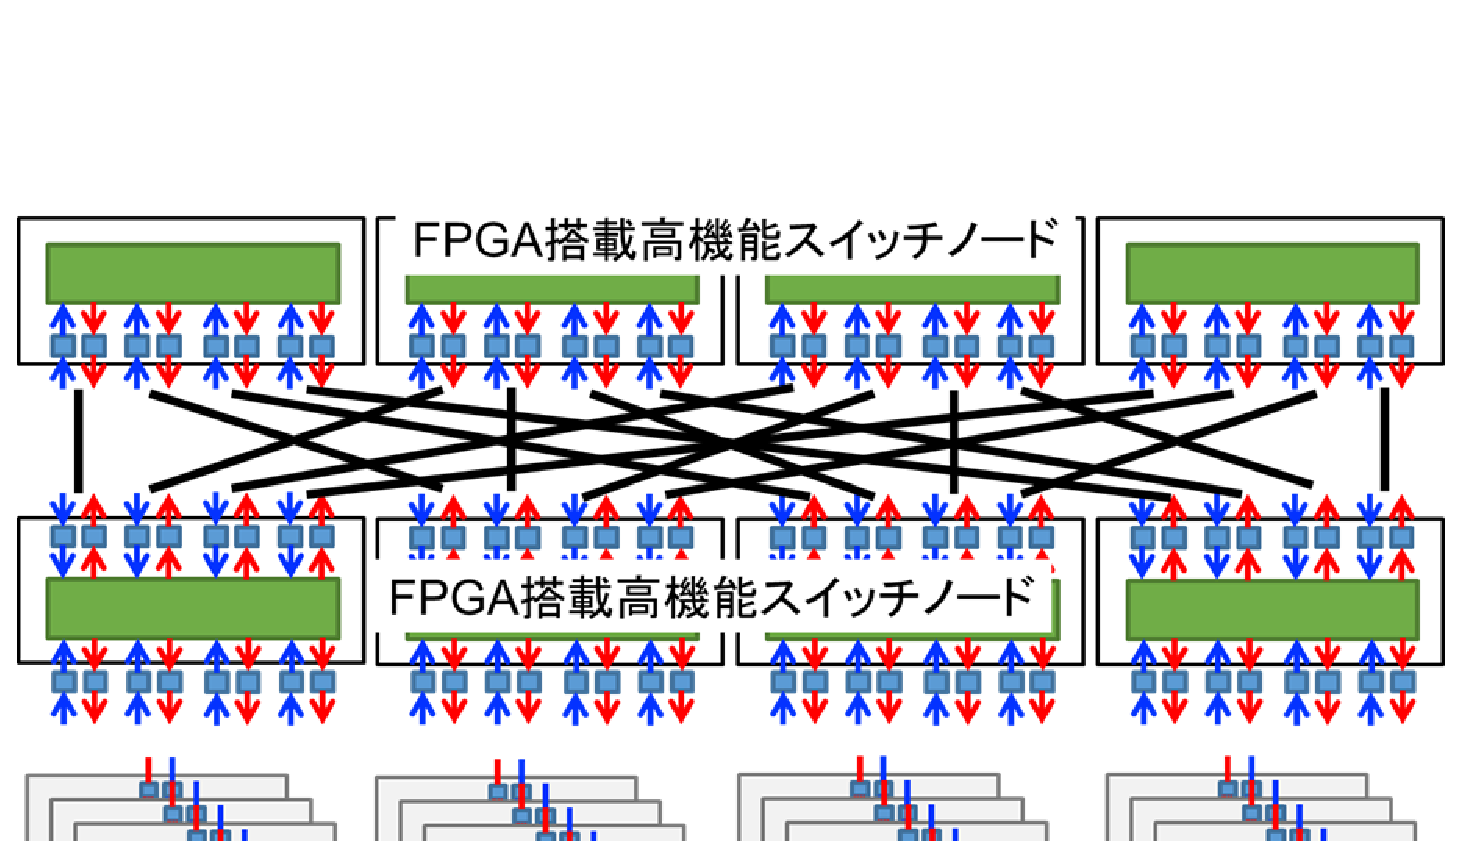
\includegraphics[width=1.0\columnwidth]{fig/FiC.eps}
  \caption{FiCの構成例}
%  \ecaption{Static analysis result of an example pattern}
  \label{fig_fic1}  
 \end{center}  
\end{figure}

\begin{figure}[ht]  
 \begin{center}   
	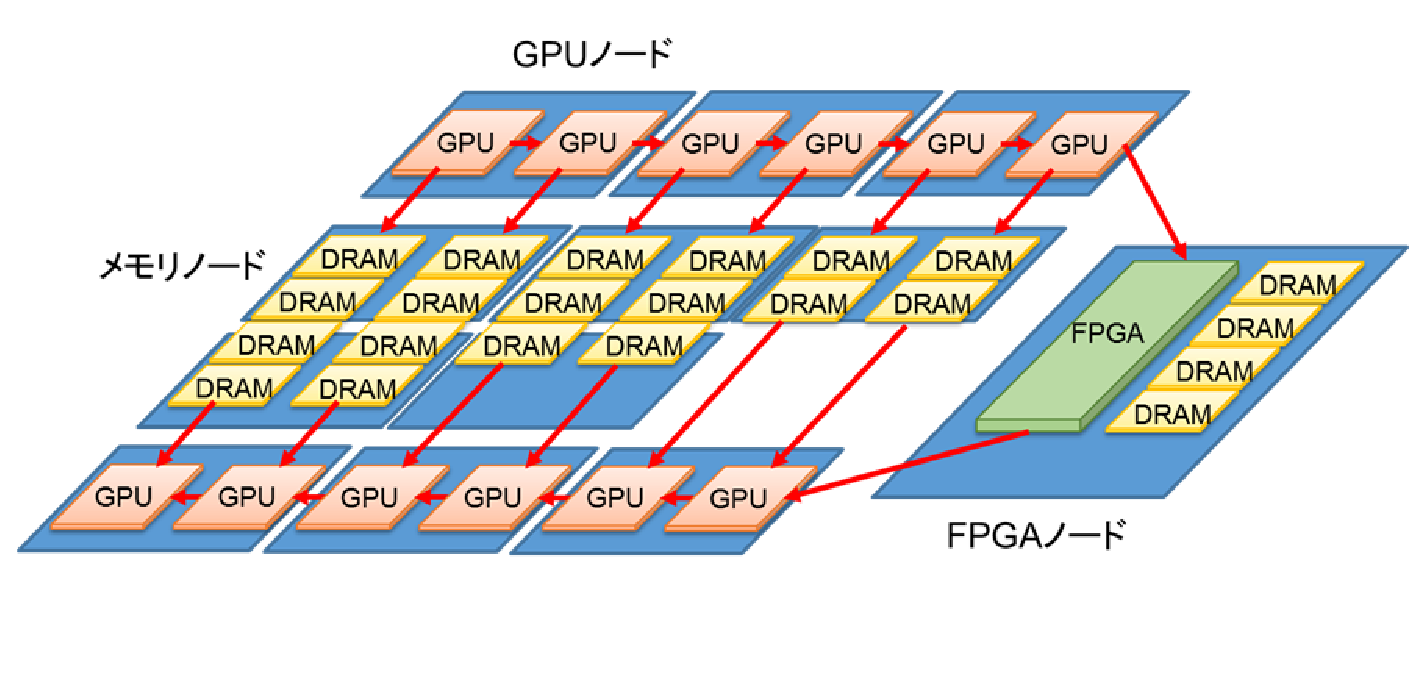
\includegraphics[width=1.0\columnwidth]{fig/example.eps}
  \caption{FiCによる学習システム構成例}
%  \ecaption{Static analysis result of an example pattern}
  \label{fig_fic2}  
 \end{center}  
\end{figure}

\section{FiC-SW1}
FiC-SW1は、初期のソフトウェア開発用のテストベッドのために使う、高速リンクを多数接続したFPGAボードである。
このFiC-SW1ボードはシステムソフトウェア開発用テストベッドとしての役割だけだでなく、
将来のFiCシステムのスイッチングハブとしての役割、GPU開発が完了するまでの演算コアとしての役割もある。


図\ref{fig_sw1}に現在開発中のFiC-SW1ボードの構成を示す。
FPGAにはXilinx社のKintex Ultrascale KU095を用いる。
ストレージとしてはDDR-4 SDRAM16GBを4組持つ。
ボード間接続のためには8Gbpsの高速光シリアルリンクを8組装備する。
リンクは全二重のため、合計の転送容量は16Gbpsとなる。

また、制御用に制御用に RaspberryPi 3 ボードをドーターボードの形で接続する。FPGAの再構成などはこのRasPi3からEthernet経由で行う。

\begin{figure}[ht]  
 \begin{center}   
	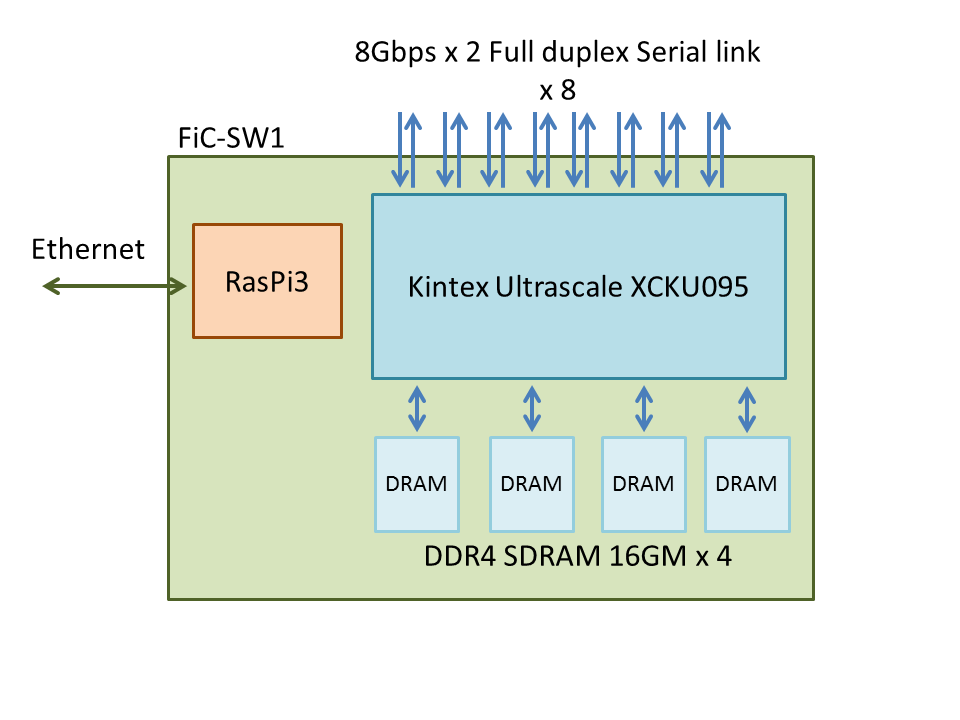
\includegraphics[width=1.0\columnwidth,bb=0 0 720 540]{img/ficsw1.png}
  \caption{FiC-SW1ボードの構成}
%  \ecaption{Static analysis result of an example pattern}
  \label{fig_sw1}  
 \end{center}  
\end{figure}

\section{FiC-SW1のサーキットスイッチング}
FiCシステムでのスイッチノードの役割も持つFiC-SW1ボードのサーキットスイッチングによる通信についてを解説する。

サーキットスイッチングとは、通信の前に事前に通信路を設定し、一定の帯域を占有してから送受信を行う通信の方式である。
FiCシステムが扱う機械学習アルゴリズムの多くは、1対1、1対全、全対全など、特定の通信路をあからじめ予測することが可能である。
そのため、通信帯域と通信遅延を保証することができるサーキットスイッチングがFiC-SW1には採用された。

図\ref{fig_switch}はFiC-SW1のスイッチの概要図である。このスイッチが1サイクルあたりに受信する転送データを格納する容量を持つバッファとして「スロット」を定義する。
そして、図\ref{fig_switch}にように入出力スロット間の接続によって経路を構成する。経路は1対1だけでなく、1対多が可能で、効率的にマルチキャストできる。
各ポートでは、1サイクルごとに順番にスロットを巡回して送受信を行うことで時分割多重(TDM : Time Division Multiplexing)を実現する。
各スロットの読み書きは同期を取らず、RAWハザード(データ書き込み前にデータ読み込みをしてしまうエラー)と、WARハザード(データ読み込み前にデータ書き換えをしてしまうエラー)のみを保証するだけで十分である。

スイッチのポートには隣接するスイッチに繋がるものと、FPGAなどの計算ノードに繋がるものが存在する。

このスイッチでは、スロットの書き込み位置によって経路が一意に決定されるよう事前に経路を設定しなければならない。
入出力スロット間の接続や再接続には、FiC-SW1内部向けに用意されたスロットへ特定の値を書き込むことで行われる。
図\ref{fig_multicast}は、1対2通信を利用してこのスロットに値を書き込み、マルチキャストへと接続を再構成している例である。
このように、定期的に入出力スロット間の接続は更新することが可能となっている。
ただし、内部向けのこのスロットは、FiC-SW1上で演算を行う際の入出力が本来の目的である。

このように、現状のFiC-SW1ボードでは光リンクと電気スイッチによってサーキットスイッチングを行う。
しかし、FiCシステムでは将来的に、光ネットワークを採用したより高速な相互通信を行う計画がある。
そのため、この電気スイッチは、光スイッチに置き変えられることを想定して設計された。
この場合、時分割多重は波長多重に置き変えられ、1スロットは1チャンネルに相当することになる。

\begin{figure}[ht]  
 \begin{center}   
	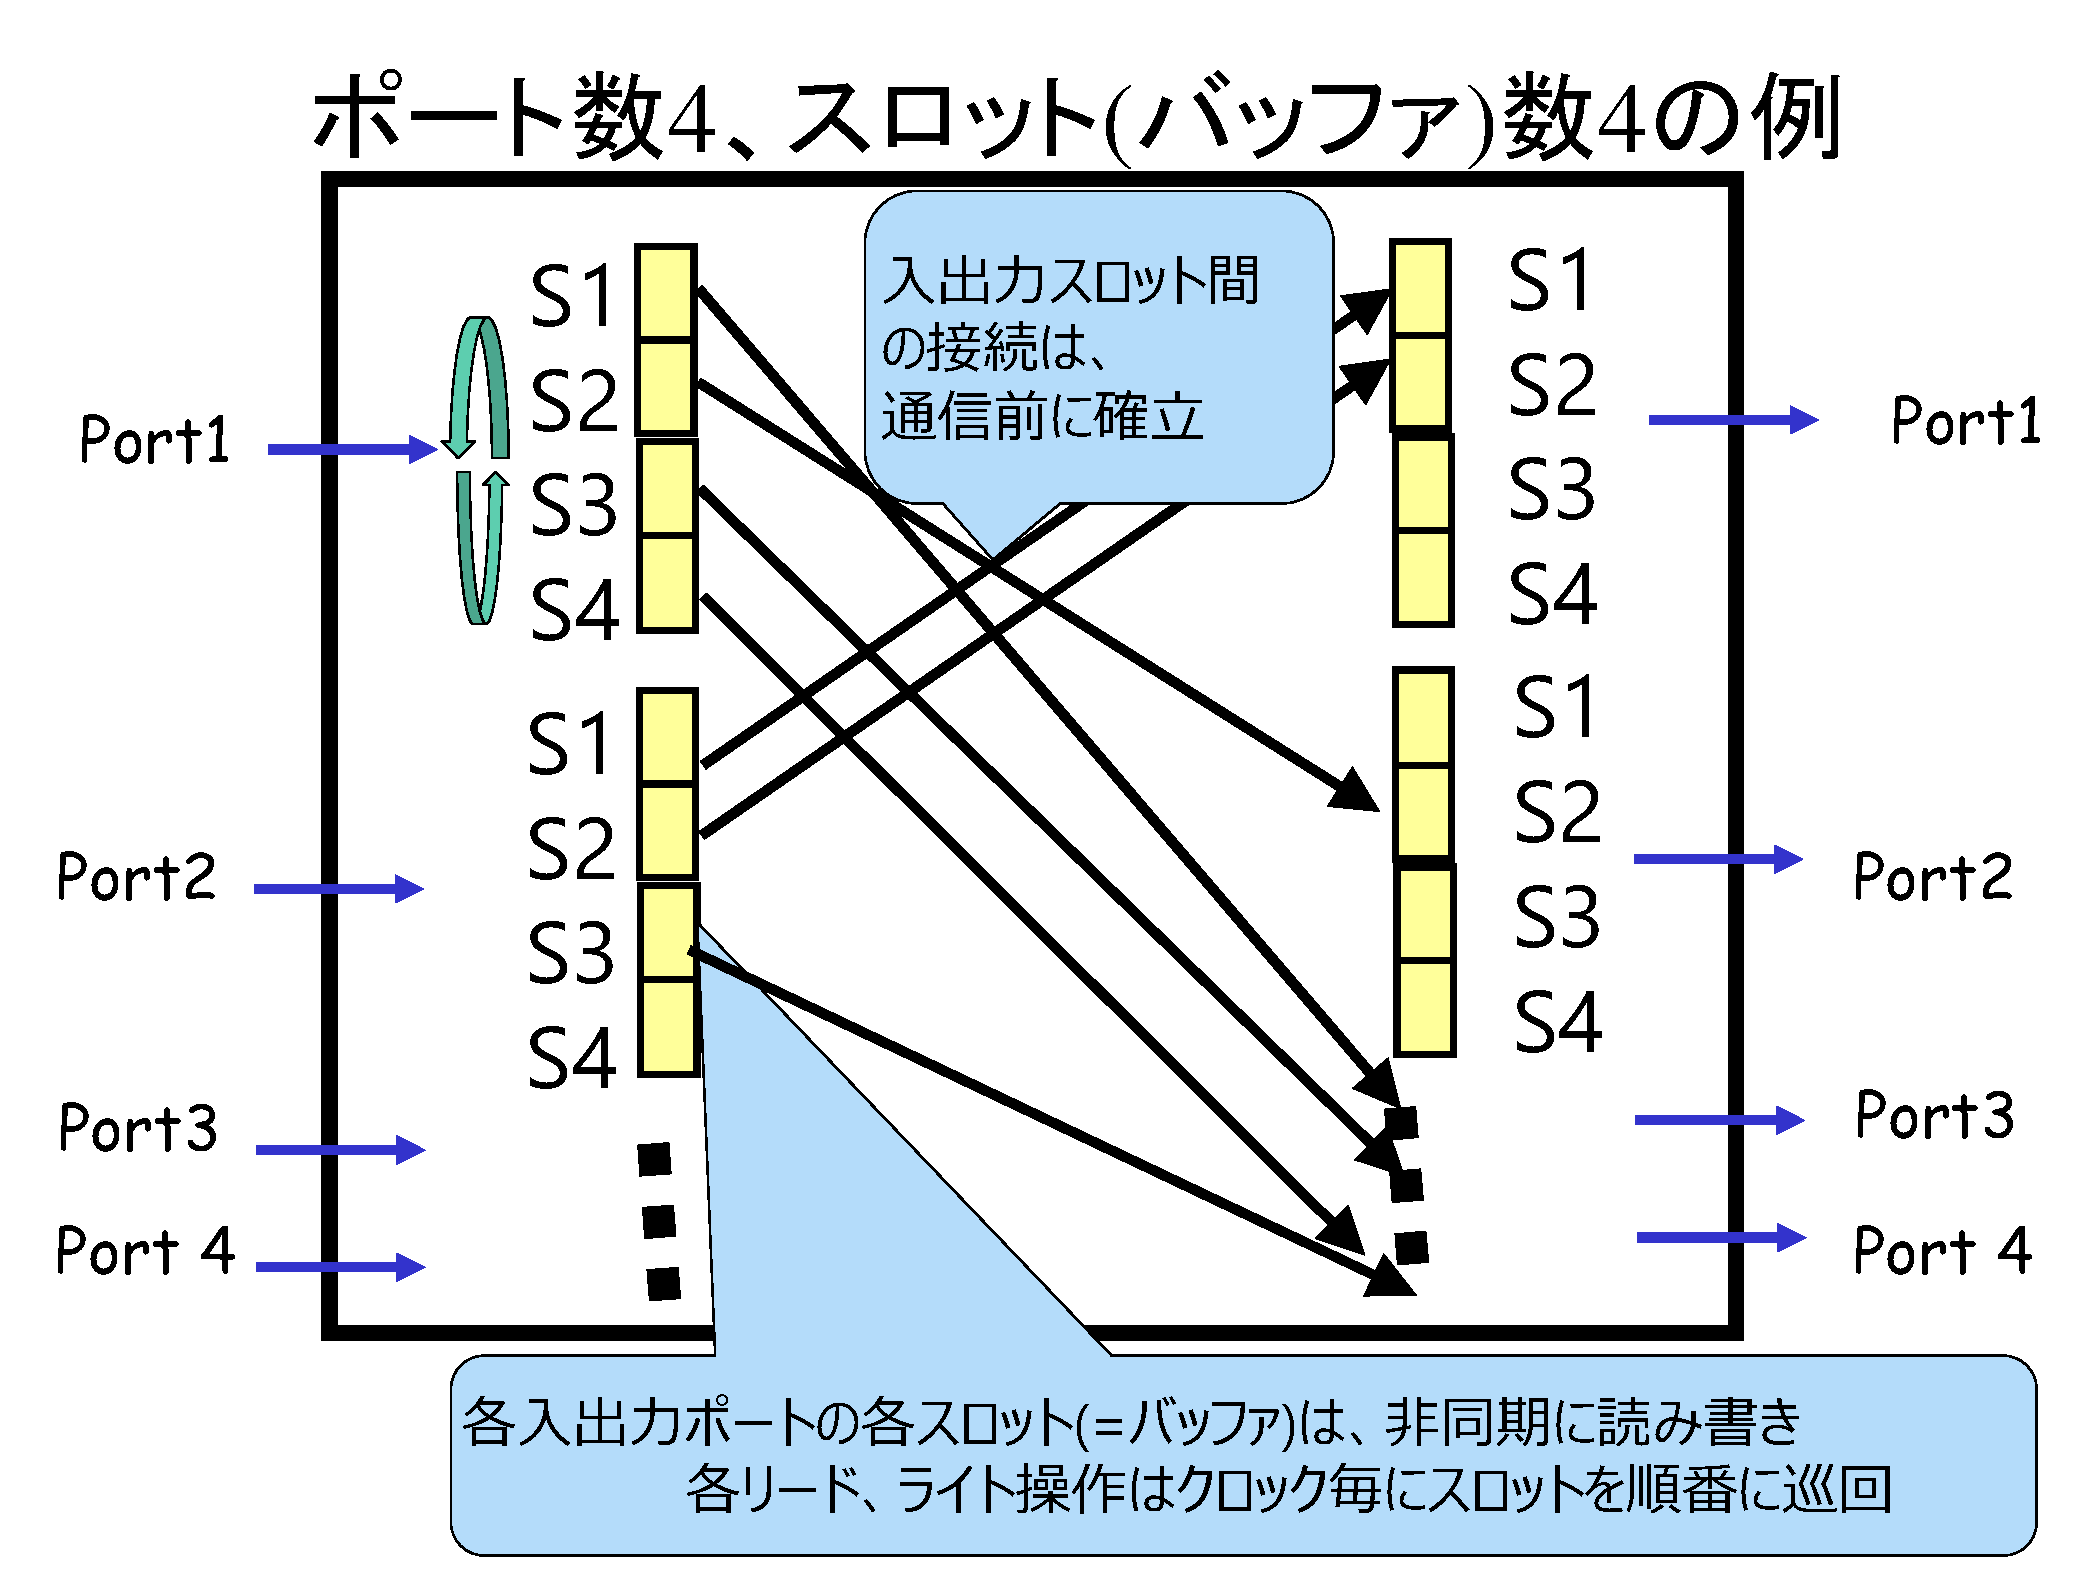
\includegraphics[width=1.0\columnwidth]{fig/switch.eps}
  \caption{FiC-SW1のサーキットスイッチ}
%  \ecaption{Static analysis result of an example pattern}
  \label{fig_switch}  
 \end{center}  
\end{figure}

\begin{figure}[ht]  
 \begin{center}   
	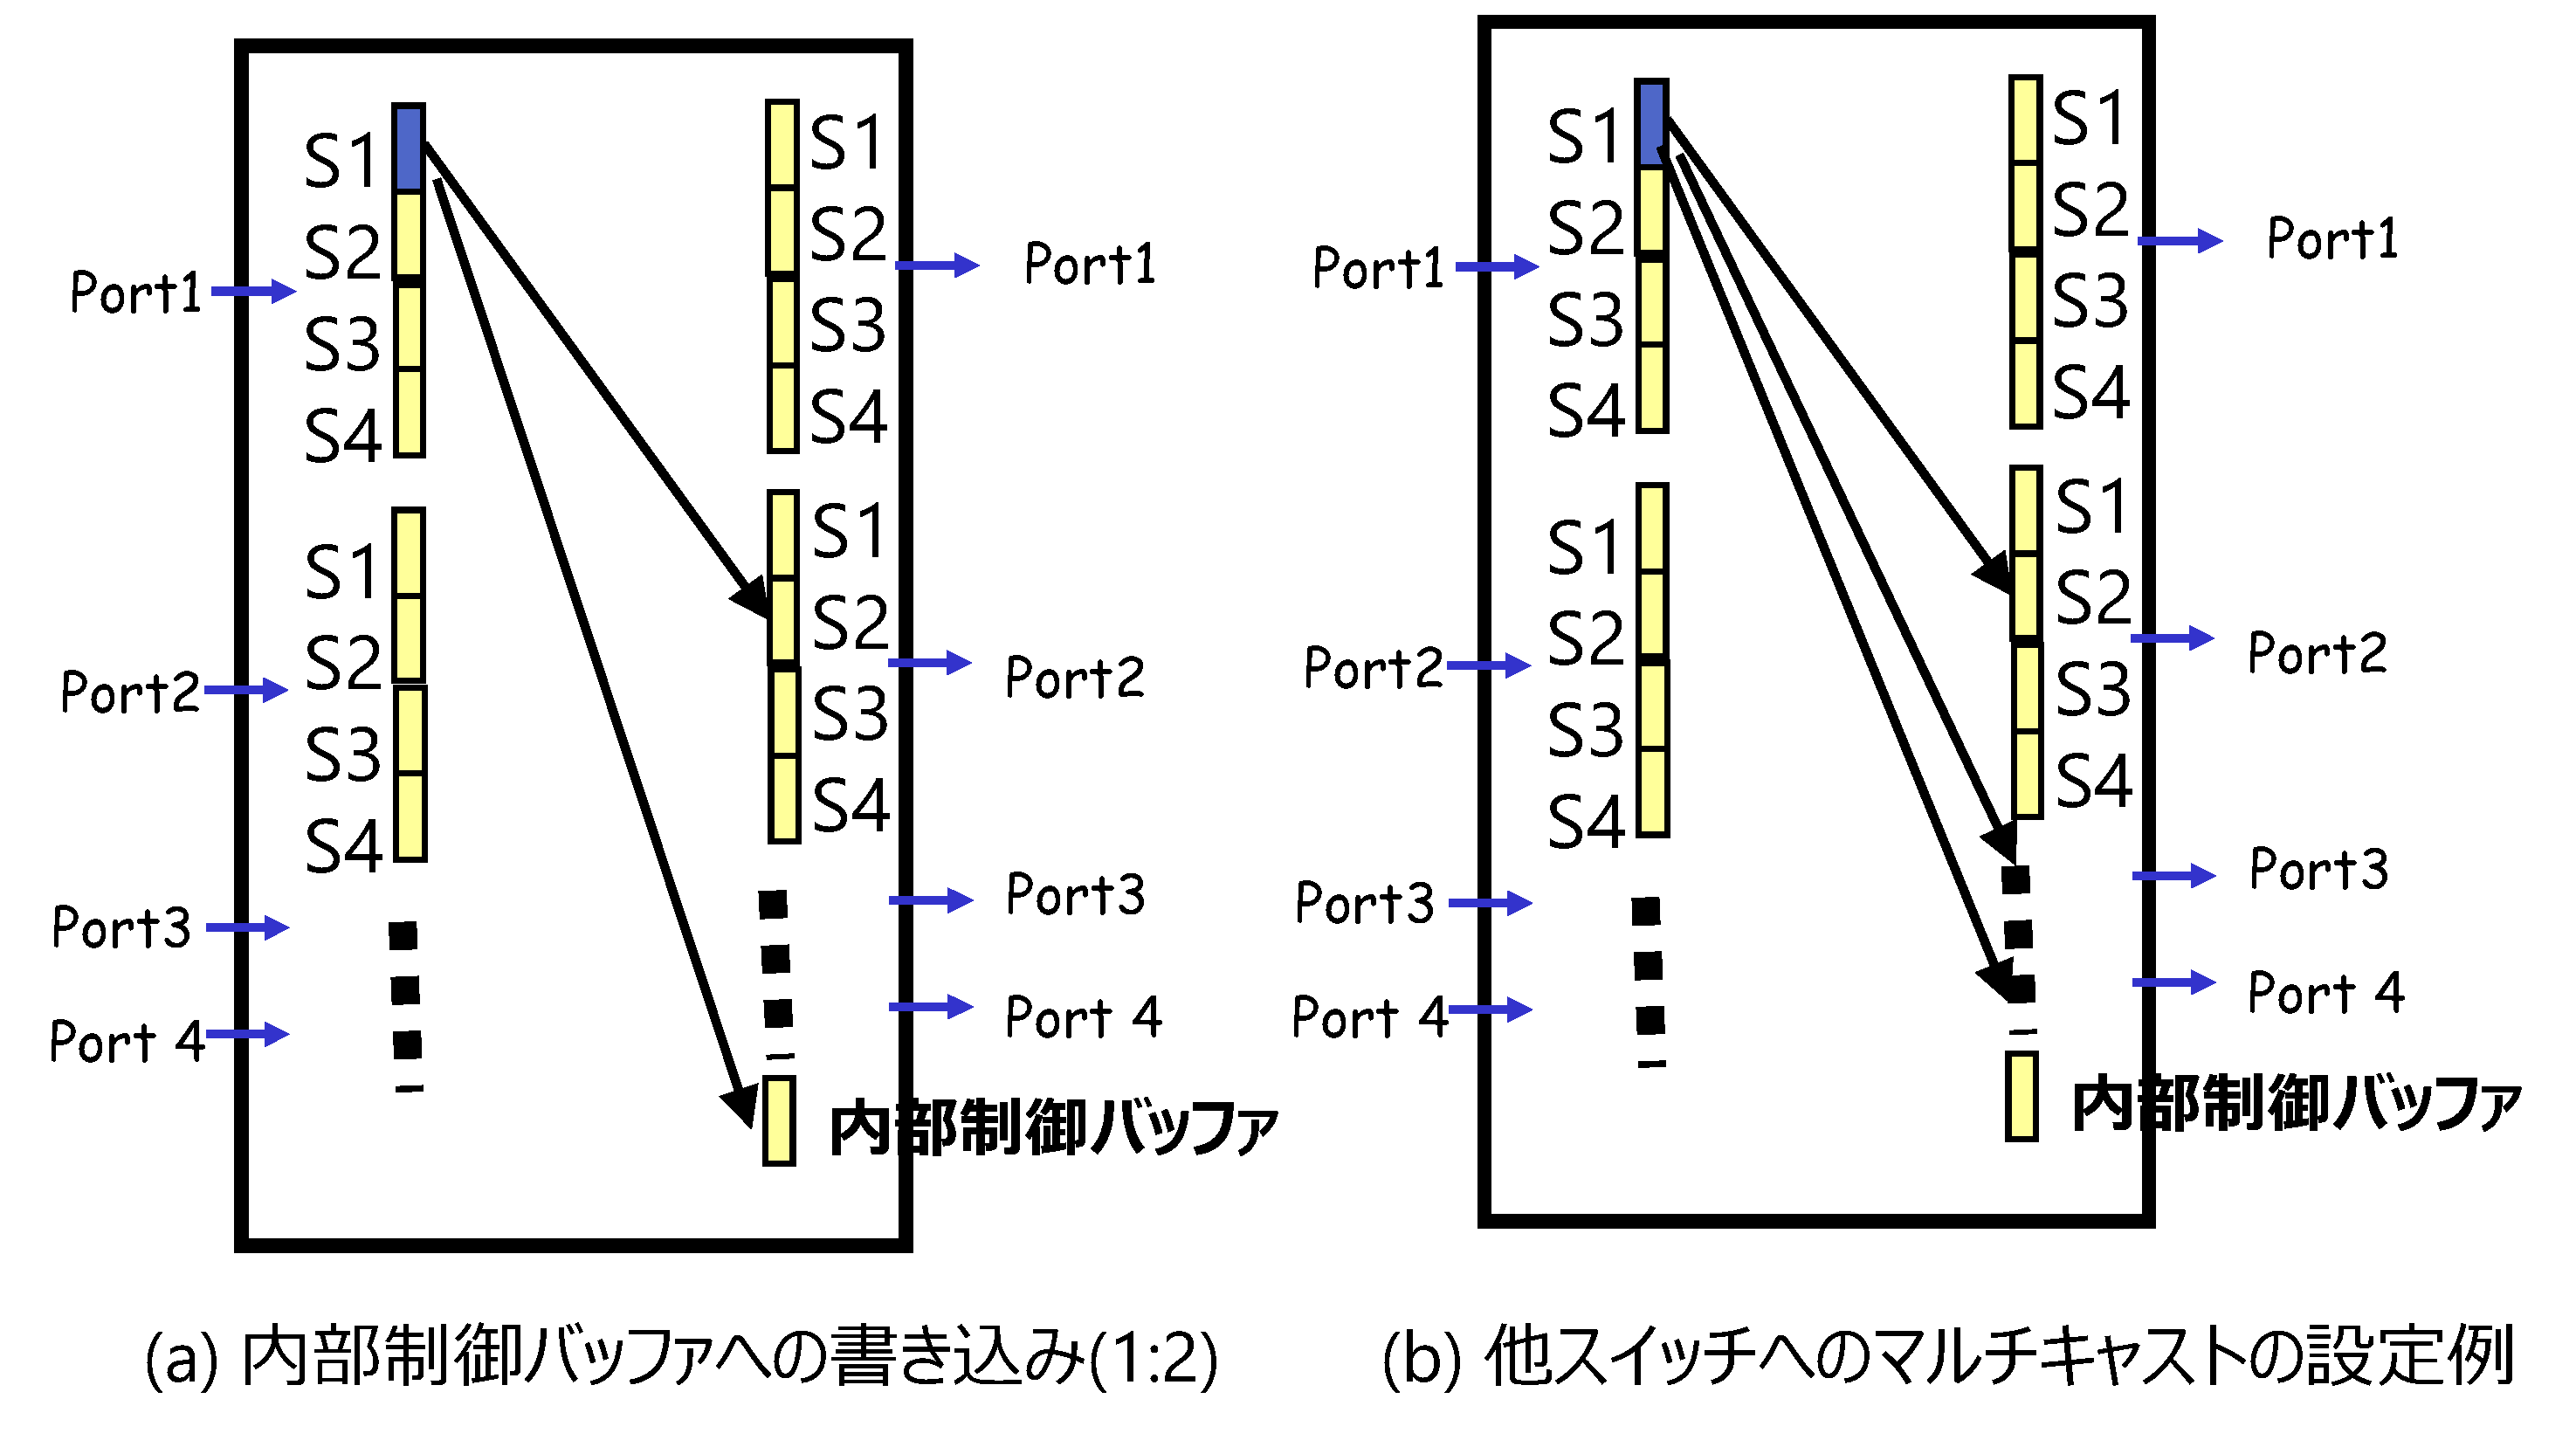
\includegraphics[width=1.0\columnwidth]{fig/multicast.eps}
  \caption{入出力スロットの再接続の例}
%  \ecaption{Static analysis result of an example pattern}
  \label{fig_multicast}  
 \end{center}  
\end{figure}


\chapter{畳み込みニューラルネットワーク(CNN:Convolutional Neural Network)}
\section{CNNの概要}
この章では、FiC-SW1の予備評価のためにベンチマークアプリケーションとして実装する畳み込みニューラルネットワーク(CNN:Convolutional Neural Network、以下CNN)について解説する。

CNNは、主に画像識別に用いられる順伝搬型ネットワークの一種である。
順伝搬型ネットワークは前の層と後ろの層が互いに全対全で結びつく全結合が一般的だが、
CNNではカーネルと呼ばれるフィルタを導入して結合に局所性を持たせている。
これにより、全結合に比べ計算処理を減らし、効率的に処理を行うことが可能となった。

図\ref{fig_cnn}に一般的な画像識別を行うCNNの推論の概要を示す。
CNNでは2次元画像データのことを特徴マップと呼び、特徴マップに対してカーネルを用いて畳み込み演算を行う畳み込み層と、
一定の範囲から値を絞るプーリング層の2種の層を組み合わせるのが構成と成っている。
畳み込み層は、カーネルと同じパターンが画像のどこに存在するかを判定する効果がある。
プーリング層は画像に写っている対象の位置感度を低下させ、位置に対する依存性を低くする効果がある。

また、ほとんどの場合において、畳み込み層は識別層の前に設けられる。
これは、複数の畳み込み層、プーリング層を組み合わせることで、識別層の入力値の数を絞り込み、
識別層の処理の負荷を軽くする狙いがあるからである。

さて、学習の処理では、教師データを用いて誤差逆伝搬法によって、畳み込み層と識別層の重みを繰り返し再計算していく形となる。
今回扱うのはこのようなCNNの推論処理のみなので、学習処理については詳しくは扱わないこととする。

\begin{figure}[ht]  
 \begin{center}   
	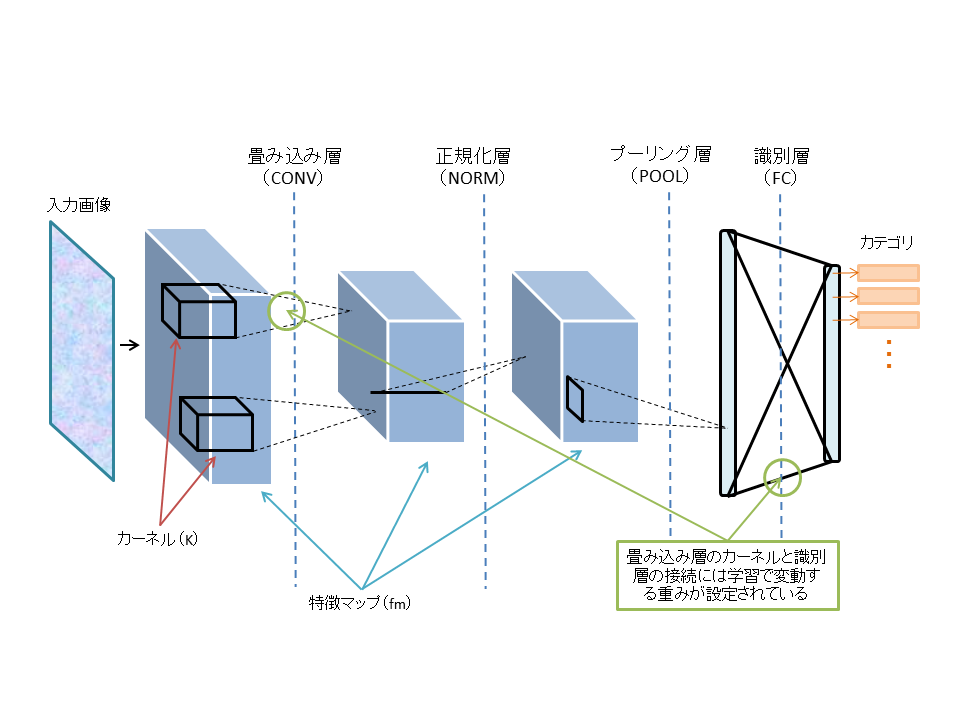
\includegraphics[width=1.0\columnwidth,bb=0 0 720 540]{img/cnn.png}
    \caption{畳み込みニューラルネットワークの推論}
%  \ecaption{Static analysis result of an example pattern}
  \label{fig_cnn}  
 \end{center}  
\end{figure}


\section{畳み込み層の処理}
CNNの特徴のひとつである畳み込み層は、入力特徴マップに対してフィルタの役割を持つカーネルを用いて畳み込み演算を行い、特徴を抽出するためのレイヤーである。

\subsection{畳み込み演算}
図\ref{fig_conv}は、畳み込み層の最も重要な処理である畳み込み演算について解説したものになる。畳み込み演算の処理は画像のフィルタリングに似ており、
N次元の入力特徴マップとN次元のカーネルの行列演算の結果を出力特徴マップの値として出力する。
カーネルの範囲K×Kは、横方向にずらしていき、端まで到達したら縦方向に
ずらしてから同様に横方向に移動させていく。このように左上から右下へとフィルタリングした結果が1枚の出力特徴マップとなる。
さらに、カーネルはM枚(チャンネル)存在し、出力特徴マップもカーネルによってM枚(チャンネル)に分かれることになる。
つまり、入力特徴マップN枚とカーネルM×N枚から出力特徴マップM枚を計算するのが畳み込み演算である。

また、畳み込み層のカーネルにはそれぞれ重みが与えられており、これが学習で変動する。つまり、M×N×K×Kが重みデータの総量となる。
さらに、畳み込み層には学習で変動するバイアス(bias)のデータが存在する。これは畳み込み演算終了後に対応する出力特徴マップに加算する数値で、
出力特徴マップのチャンネル別にM個のデータがある。


\begin{figure}[ht]  
 \begin{center}   
	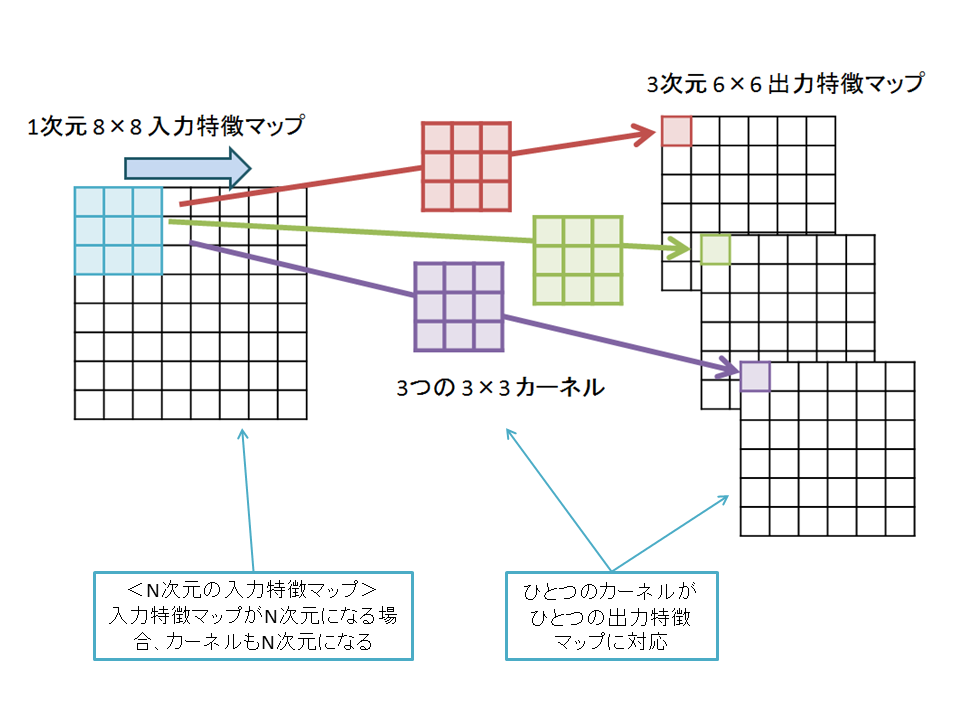
\includegraphics[width=1.0\columnwidth,bb=0 0 720 540]{img/conv.png}
    \caption{畳み込み層の演算}
%  \ecaption{Static analysis result of an example pattern}
  \label{fig_conv}  
 \end{center}  
\end{figure}

畳み込み演算を数式で表すと以下のようになる。

\[
  output(tr, tc)^{to} = \sum_{ti=0}^{N} \sum_{i=0}^{K} \sum_{j=0}^{K} weight_{to, ti}(i, j) * in(S * tr + i, S * tc + j)^{ti}
\]

このように、フィルタリング処理と同様、畳み込み演算は大規模な積和演算として捉えることができる。また、この演算を擬似コードで表すと以下のようになる。
コードを見るとわかるように、このデータ処理では、出力特徴マップのデータ間ではデータ並列性が存在するため、
並列演算器によって高速化できる余地があることがわかる。
このことは今回の畳み込みアクセラレータの実装を検討する上で最も重要な事実となる。

\begin{itembox}[1]{畳み込み演算のCコード}
\begin{verbatim}
for (int tr = 0; tr < R; tr++)
  for (int tc = 0; tc < C; tc++)
    for (int to = 0; to < M; to++)
      for (int ti = 0; ti < N; ti++)
        for (int i = 0; i < K; i++)
          for (int j = 0; j < K; j++)
            output[to][tr][tc] +=
              input[ti][S*tr+i][S*tc+j] *
              weight[to][ti][i][j];
\end{verbatim}
\end{itembox}

\subsection{活性化関数}
さて、畳み込み層ではもうひとつ重要な処理が行われる。それは畳み込み演算の結果を活性化関数と呼ばれる関数にかける処理である。
活性化関数は畳み込み演算の結果を正規化する目的で行われる計算で、正規化線形関数(ReLU : Rectified Liner function)やシグモイド関数などが使われる。

たとえば、最も一般的な正規化線形関数は数式にすると以下のようになる。

\[
  f(u) = max(u, 0)
\]

この関数は他の関数に比べ、処理が単純で、入力の変動が大きさに対して寛容なため、近年のニューラルネットワークで使われる機会が多い。

\section{その他の層の演算}
今回は畳み込み層の処理を主なベンチマークとして扱うが、CNNには他にもプーリング層や正規化層、識別層が存在している。ここではそれらの層の処理について解説する。

プーリング層(POOL)では、主に特徴の位置感度を低下させる目的で、最大値プーリング(maxpooling)や平均値プーリングが行われる。
たとえば、最大値プーリングでは、プーリングの範囲P×Pの中で最も大きい値を抽出し、出力とする。P×Pの範囲が大きいほど特徴マップのサイズは
小さくなって出力されることになる。

正規化層(NORM)では、画像のコントラストや露出の影響を抑え、識別の精度をあげる目的で設置される。
ここでは局所コントラスト正規化(LRN : Local Response Normalization)を解説する。

LRNはAlexNetの正規化層で用いられる処理で、数式で表すと以下のようになる。

\[
  output(x, y)^{i} = input(x, y)^{i} / (k + \alpha \sum_{j=max(0, i-n/2)}^{min(N-1, i+n/2)} (a^j_{x, y})^2)^\beta
\]

k、n、$\alpha$、$\beta$がパラメータであり、たとえば、AlexNetの正規化層では、k=1、n=5、$\alpha$=?、$\beta$=?となっている。

識別層(FC)は純粋な順伝搬型ニューラルネットワークであり、
すべての入力値と出力値の間に重みとバイアスが与えられている全結合の形になっている。
この重みは畳み込み層の重み・バイアスと同様、学習によって変動する。
畳み込み層、プーリング層、正規化層を経て抽出さえた値はこの識別層によって
最終的な分類が行われる。

識別層の処理を数式で表すと以下のようになる。

\[
  output(i) = bias(i) + \sum_{j=0}^{N} weight(i, j) * input(j)
\]

\section{大規模な画像識別CNN : AlexNet}
AlexNet\cite{alexnet}はImageNet2012で発表され、現在のCNNの基礎となっている一般的な
画像識別ニューラルネットワークのひとつである。
5つの畳み込み層、3つのプーリング層、2つの正規化層、3つの識別層(全結合層)から成る
このCNNは、227×227ピクセルのカラー画像を1000のカテゴリに分類することができる。
図\ref{imagenet_img}はAlexNetの全体の流れを示している。

今回はこのAlexNetの畳み込み層の推論(順伝搬)をベンチマークアプリケーションとして扱う。
表\ref{imagenet}は今回利用するAlexNetの各層のパラメータをまとめたものである。
Nは入力特徴マップの次元数、Mは出力特徴マップの次元数、R、Cは出力特徴マップサイズ、Kはカーネルサイズ、Sはストライド、padはパディングのパラメータとなる。
パディングとは畳み込み演算を行う前に、入力特徴マップの周りを0で埋める操作である。

一般的に畳み込み層はCONV、プーリング層はPOOL、正規化層はNORM、識別層はFCと略され、後ろに
その層が何層目にあたるかの数字をつけて区別する。

実際に2012年に発表されたAlexNetでは、CONV1、CONV2、CONV5は独立した2つのグループに分けられていた。
たとえば、CONV1の出力特徴マップは前半48層と後半48層といったように半分に分けられる。
しかし、今回の実装ではそれをひとつに結合したものを扱う。AlexNetがこのような2つのグループに
分かれていたのは、2つのGPUで処理を分担する都合上であり、それをひとつのシステム上で処理できるならば
ひとつのグループにまとめてしまっても問題はないためである。

\begin{figure}[ht]  
 \begin{center}   
	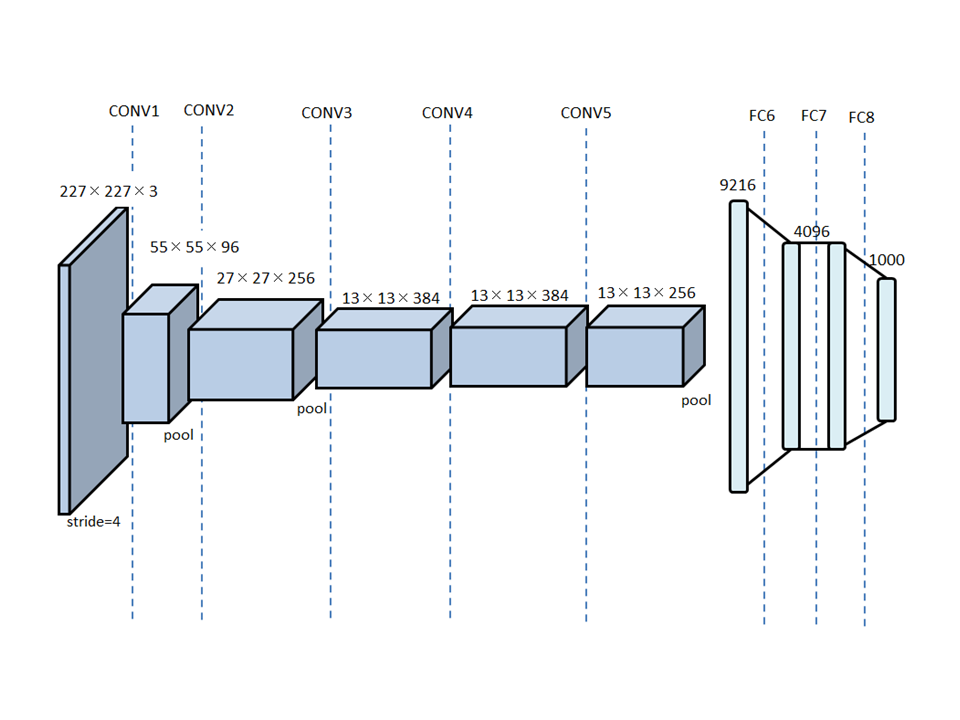
\includegraphics[width=1.0\columnwidth,bb=0 0 720 540]{img/imagenet.png}
    \caption{AlexNet\cite{alexnet}の概要}
%  \ecaption{Static analysis result of an example pattern}
  \label{imagenet_img}  
 \end{center}  
\end{figure}

\begin{table}[ht]
 \begin{center}
  \caption{AlexNetの各層の詳細なパラメータ}
   \begin{tabular}{|c|c|c|c|c|c|c|} \hline
     層 & 入力fm N & 出力fm M & サイズ(R,C) & カーネルK & ストライドS & パディング \\ \hline
     CONV1 & 3 & 96 & 55 & 11 & 4 & 0 \\
     NORM1 & 96 & 96 & 55 & - & - & - \\
     POOL1 & 96 & 96 & 27 & 3 & 2 & - \\
     CONV2 & 96 & 256 & 27 & 5 & 1 & 2 \\
     NORM2 & 256 & 256 & 27 & - & - & - \\
     POOL2 & 256 & 256 & 27 & 3 & 2 & - \\
     CONV3 & 256 & 384 & 13 & 3 & 1 & 1\\
     CONV4 & 384 & 384 & 13 & 3 & 1 & 1\\
     CONV5 & 384 & 256 & 13 & 3 & 1 & 1\\
     POOL5 & 256 & 256 & 6 & 3 & 2 & - \\
     FC6 & 9216 & 4096 & - & - & - & - \\
     FC7 & 4096 & 4096 & - & - & - & - \\
     FC8 & 4096 & 1000 & - & - & - & - \\ \hline
  \end{tabular}
  \label{imagenet}  
 \end{center}
\end{table}

\chapter{関連研究}
\section{マルチFPGAシステムでのボード間通信}
有名なマルチFPGAシステムとしては、たとえば、Microsoft社の提供するBing検索エンジンに利用されている
Catapult\cite{Catapult}がある。Catapultでは、ボード間の接続にSerial Attached SCSIの物理層を用いた
独自のシリアルI/Oを装備している。
また、EthernetやPCIeを使う例としては、Berkeley Univ.のBEE3\cite{BEE3}、EthernetとInfinibandを使う例として、
Imperial CollegeのAXCEL\cite{Axcel}がある。国内の例では、たとえば、東北大学の密結合クラスタ\cite{Sano}も
Ethernetの物理層を利用している

これらのマルチFPGAシステムはすべてパケット交換方式によってボード間の通信を行っている点で、
回線交換方式のFiCシステムとは異なっている。
%マルチFPGAシステムのボード間接続は、EthernetなInfinibandなどの標準インタフェースを
%用いる例が多い。Berkeley大学のBEE3\cite{BEE3}は、ボード上のFPGAはパラレルI/Oを用いているが
%ボード間の接続はEthernetやPCIeを用いており、Imperial CollegeのAXCEL\cite{Axcel}も
%FPGAボード間の
%接続は、EthernetとInfinibandであり、
%東北大学の密結合クラスタ\cite{Sano}もEthernetの物理層を利用している。独自の
%シリアルI/Oを用いたシステムとしてはMicrosoftのCatapult\cite{Catapult}があり、
%Serial Attached SCSIの物理層を利用している。これらのすべてのマルチFPGAシステムでは
%パケット転送を用いており、STDMを用いているCiFとは全く異ったネットワークである。

\section{大規模畳み込みニューラルネットワーク}
今回の検証ではAkexNet\cite{alexnet}をベンチマークとして使用したが、近年
注目されている比較的小規模な畳み込み層を何層も重ねた形の
GoogLeNet\cite{googlenet}やResNet\cite{resnet}についても検討しなければ
ならない。一般的には深いネットワークのほうがパラメータ数が少なくなる傾
向があり、この期もその傾向が続く場合はハードウェアデザインに大きな影響
を与える可能性がある。ただし、これに関しては反論\cite{dodeepnet}もある。

\section{FPGAベースのCNNアクセラレータ}
CNN、もしくはより汎用的なニューラルネットワークの処理を大規模なシステ
ムによって高速化、省電力化する代表的な研究としてDaDianNaoマシ
ンラーニングスーパーコンピュータ\cite{dadiannao}が挙げられる。
これは推論学習のミリ秒単位での高速化に焦点を当てたプロジェクトで、重みデータを可能な限り
ローカルに保存できるような設計をしている。それによってメモリ帯域幅のボトルネックを
改善するというコンセプトではFiCプロジェクトとも関連が強い。
%これは識別学習のミリ秒単位での高速化に焦点をあてたプロジェクトで、重みデータを可能な限りローカルに保存できるような設計をし、メモリバンド幅のボトルネックを解消するというコンセプトでは我々のプロジェクトとも関連性が強い。
ただし、\cite{dadiannao}はASICチップシステムであり、FPGA-GPUシステムを用いる点では異なっている。



CNNに対するFPGAを用いた高速化の最初期の研究としては、2009年のCNP \cite{cnp}が挙げられる。
これはソフトウェア実行を中心としながら、畳み込み演算のフィルタリング処理をハードウェアで高速化したものである。
2010年にはFPGA上で完全なCNN実装\cite{NEC_Labs_America1}\cite{NEC_Labs_America2}\cite{NEC_Labs_America3}が行えるようになった。

現在、FPGAベースのCNNアクセラレータはUCLAのマルチレイヤーCNNアクセラレータ\cite{fpgaopt}が有名である。
今回実装を行ったアクセラレータの演算部はこの設計を参考にした。

他にも、Microsoft社のCatapultのFPGAで動作するCNNアクセラレータ\cite{ms_fpgacnn}が挙げられる。
このCatapultのアクセラレータはULCAの設計を参考に、CatapultサーバとAria10を組み合わせて3倍以上の性能向上を実現している。





\chapter{目的}
本稿は、FiC-SW1ボード上のFPGAにCNNの畳み込み層の処理をする並列畳み込みアクセラレータを実装し、
その計算時間と通信時間の割合をシミュレーションによって測定することが目的である。そのためには、
以下の2つの課題に取り組まなくてはならない。畳み込み層の並列化と相互通信の検討については第6章、
畳み込みアクセラレータの実装については第7章で扱う。

\begin{description}
 \item[畳み込み層の並列化と相互通信の検討]\mbox{}\\ 
	    大規模な畳み込み演算を複数のFiC-SW1ボード上で処理するために最適なタスク分割を行う。
	    また、畳み込み演算を分割処理するにあたって相互通信が必要になる。その相互通信量と時間コストを静的に計算する。
 \item[畳み込みアクセラレータの実装]\mbox{}\\
	    分割された畳み込み演算を高速に行うために、FiC-SW1ボード上のFPGAに畳み込みアクセラレータの実装を行う。
\end{description}




\chapter{畳み込み層並列化と相互通信についての検討}
\section{概要}
この章では、まず、マルチFiC-SW1システム上でCNNを扱うために畳み込み層の並列化を行う。
そして、その並列畳み込み演算をFiC-SW1上に実装した場合の相互通信について検討する。

\cite{fpgaopt}によれば、識別時において、畳み込み層での演算は全体の実行時間の90%以上を占めることがわかっている。
今回の実装では特にこの畳み込み演算をマルチFiC-SW1システムによって高速化することを重要な課題とした。

\section{畳み込み層の並列化}
畳み込み層の演算は多くの場合において、高いデータ並列性があるため、様々な並列化方式を考えることができる。

今回は、ほかの多くのニューラルネットアクセラレータ\cite{fpgaopt}\cite{dadiannao}と同様に、
入出力の特徴マップを相互通信し、重みデータをローカルストレージに保存する戦略をとった。
これは、特徴マップの計算量が(M×R×C)であるのに対して重みは(M×N×K×K)で、
一般的なCNNでは重みのほうが計算量が多くなる傾向があり、特徴マップを相互通信するほうが低コストになるからである。

図\ref{fig_paraconv}はCONV1を例に、今回の戦略で畳み込み層を16並列化したときのタスク分割の様子を示している。
AlexNetのCONV1は[3, 227, 227]のサイズの入力特徴マップから、[96, 3, 11, 11]のサイズの重みを用いて、
[96, 55, 55]のサイズの特徴マップを出力するものである。これを16並列化すると、重みが16分割されるため、1ノードあたりの
重みは[6, 3, 11, 11]となる。それに伴って、出力特徴マップのサイズも16分の1になるため、[6, 55, 55]となる。
ただし、この16分の1の出力は次の層のために全対全の相互通信によって共有しなければならない。

図\ref{fig_cnn_broadcast}はAlexNetを並列化した際に、どのタイミングで特徴マップ共有のための全対全通信が必要になるかを示している。
基本的には、ひとつの畳み込み層・識別層に対して1回の共有をしなければならない。また、正規化層の前でも共有が必要に
なるが、これはLRNの演算で使う前後2チャンネル分の特徴マップに対してのみであり、全対全通信と比べて遥かに小さいため、今回は詳しくは扱わない。

以下は、並列化された畳み込み演算を疑似コードで表したものになる。Tmの値によって並列度が変化し、たとえば、M=96のCONV1を16並列化
した場合、Tm=6となる。

\begin{itembox}[1]{出力特徴マップチャンネルで並列化された畳み込み演算のCコード}
\begin{verbatim}
for (int tr = 0; tr < R; tr++)
  for (int tc = 0; tc < C; tc++)
    for (int to = 0; to < M; to += Tm) //Tmごとに出力を分割
      for (int ti = 0; ti < N; ti++)
        for (int i = 0; i < K; i++)
          for (int j = 0; j < K; j++)
            output[to][tr][tc] +=
              input[ti][S*tr+i][S*tc+j] *
              weight[to][ti][i][j];
\end{verbatim}
\end{itembox}
						
						
\begin{figure}[ht]  
 \begin{center}   
	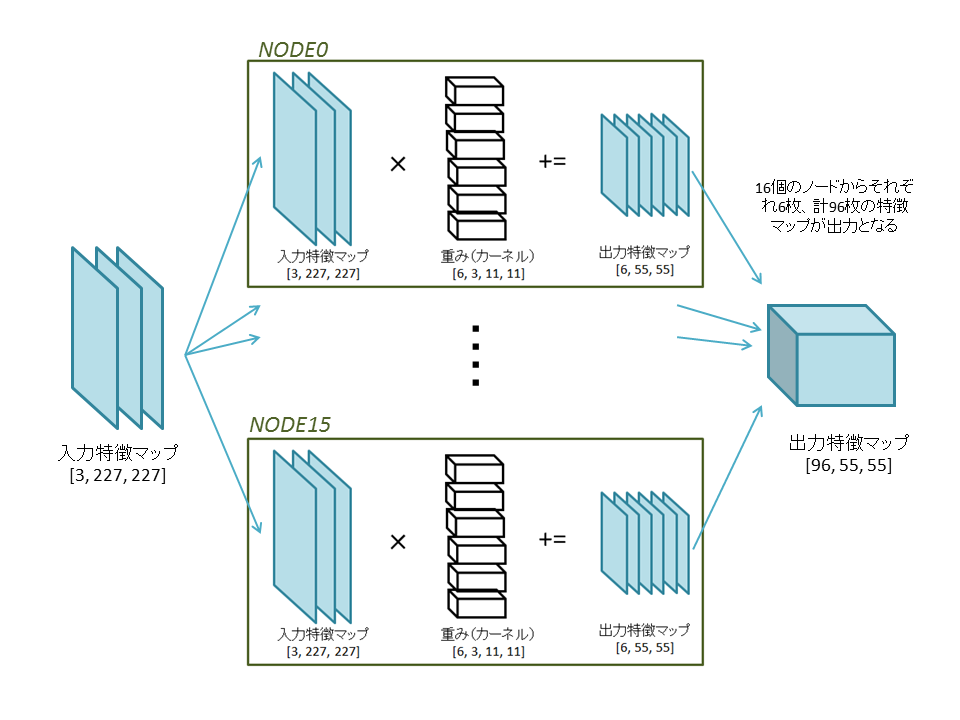
\includegraphics[width=1.0\columnwidth,bb=0 0 720 540]{img/paraconv.png}
  \caption{16並列化されたCONV1の畳み込み演算の例}
%  \ecaption{Static analysis result of an example pattern}
  \label{fig_paraconv}  
 \end{center}  
\end{figure}

\begin{figure}[ht]  
 \begin{center}   
	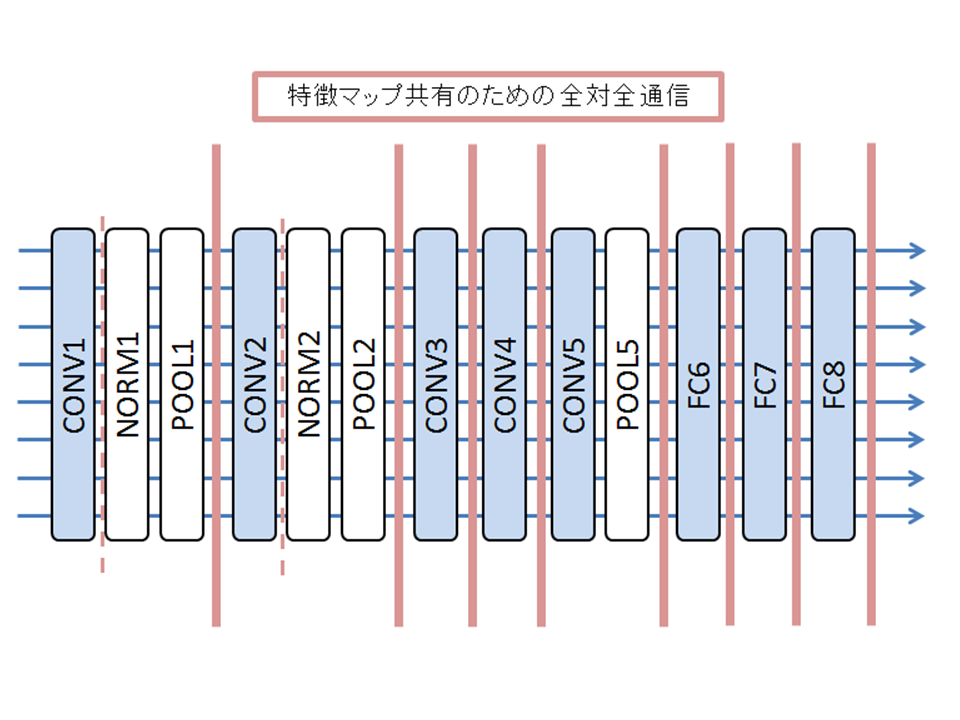
\includegraphics[width=1.0\columnwidth,bb=0 0 720 540]{img/cnn_broadcast.png}
  \caption{並列化されたAlexNetにおける特徴マップ共有のタイミング}
%  \ecaption{Static analysis result of an example pattern}
  \label{fig_cnn_broadcast}  
 \end{center}  
\end{figure}

\section{マルチFiC-SW1システム上での並列化された畳み込み層の扱い}
さて、並列畳み込み演算をマルチFiC-SW1システム上での処理に置き換えると、1ノードをひとつのFiC-SW1ボードに置き換えるのが妥当である。
重みはFiC-SW1上のFPGAのメモリ資源かDRAMをローカルストレージとして用いて保存する。
また、入出力特徴マップのためもバッファを設けて、必要に応じてサーキットスイッチネットワークを利用してブロードキャストする形になる。

図\ref{fig_cnn_on_sw1}はFiC-SW1ボード上での畳み込み層の演算について解説している。
まず、演算に必要な入力特徴マップがブロードキャストによって送信されてくるまで待機しなければならない。
データが揃ったならローカルストレージの重みを用いて畳み込み演算を行い、その間はサーキットスイッチからは空データを受信し続ける。
計算が終わったら、その出力特徴マップをブロードキャストする。すべてのFiC-SW1は基本的には非同期的に動作するが、
すべてのノードがブロードキャストし終えないと次の層の処理を始めることができないため、このタイミングで同期が取られる。

さて、表\ref{node}に、このシステムでAlexNetを実装した際のひとつのFiC-SW1あたりの出力特徴マップ数とブロードキャストされるデータ量を
算出した結果を示す。並列度が高くなるほど1ノードが扱う出力特徴マップ数が減っていることがわかる。しかし、たとえば、CONV1の結果を見ると、
16並列から64並列では並列度は4倍になっているのに対して、出力特徴マップ数は6チャンネルから2チャンネルと4分の1にはなっていない。
CONV1の出力特徴マップ数96は、64で割り切れないため、最適なタスク分割を行えていないことが理由である。
このように畳み込み層の出力特徴マップ数によっては、過剰な並列化は通信の無駄を増やしてしまうことに注意しなければならない。

\begin{figure}[ht]  
 \begin{center}   
	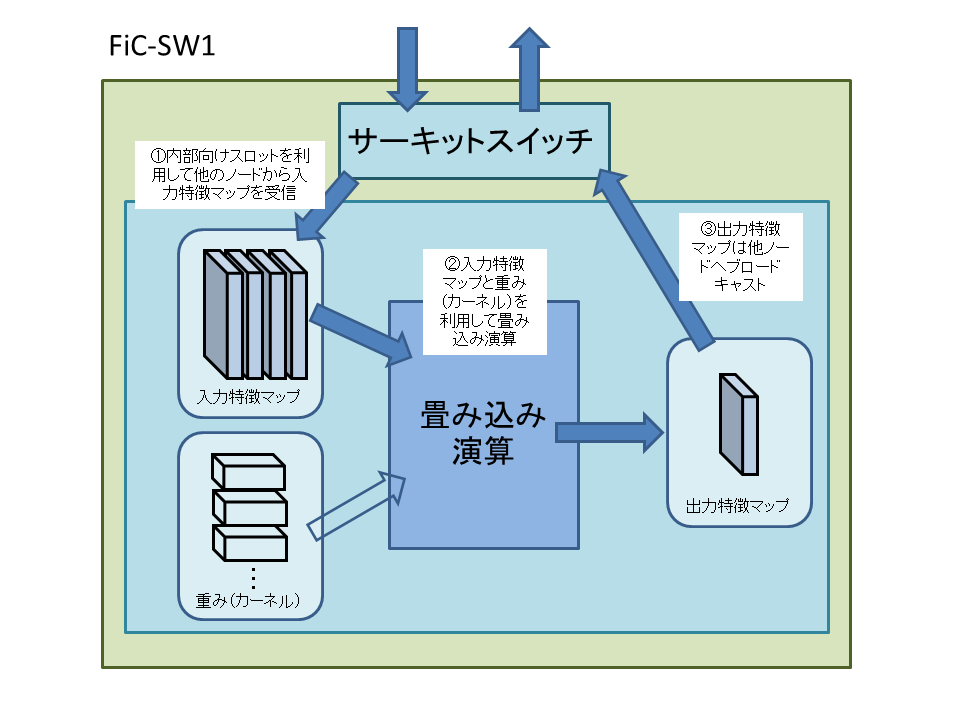
\includegraphics[width=1.0\columnwidth,bb=0 0 720 540]{img/cnn_on_sw1.png}
  \caption{FiC-SW1上のCNNの計算処理の流れ}
%  \ecaption{Static analysis result of an example pattern}
  \label{fig_cnn_on_sw1}  
 \end{center}  
\end{figure}

\begin{table}[ht]
 \begin{center}
  \caption{マルチノードCNNの1ノードあたりの出力特徴マップ数とそのデータ量}
   \begin{tabular}{|c|c|c|c|c|c|c|c|c|} \hline
     & \multicolumn{2}{|c|}{4並列} & \multicolumn{2}{c|}{16並列} & \multicolumn{2}{c|}{64並列} & \multicolumn{2}{c|}{265並列}\\ \hline
     & fm & (Kb) & fm & (Kb) & fm & (Kb) & fm & (Kb) \\ \hline
     CONV1 & 24 & 559.9 & 6 & 140.0 & 2 & 46.6 & 1 & 23.3 \\
     CONV2 & 64 & 346.1 & 16 & 86.5 & 4 & 21.6 & 1 & 5.4 \\
     CONV3 & 96 & 519.2 & 24 & 129.8 & 6 & 32.4 & 2 & 10.8 \\
     CONV4 & 96 & 519.2 & 24 & 129.8 & 6 & 32.4 & 2 & 10.8 \\
     CONV5 & 64 & 73.7 & 16 & 18.4 & 4 & 4.6 & 1 & 1.2 \\
     FC6 & 1024 & 32.8 & 256 & 8.2 & 64 & 2.0 & 16 & 0.5 \\
     FC7 & 1024 & 32.8 & 256 & 8.2 & 64 & 2.0 & 16 & 0.5 \\
     FC8 & 250 & 8.0 & 63 & 2.0 & 16 & 0.5 & 4 & 0.1 \\ \hline
  \end{tabular}
  \label{node}  
 \end{center}
\end{table}

\section{FiC-SW1ネットワークによる特徴マップ共有}
図\ref{gra_broadcast_time}は、表\ref{node}を基に、出力特徴マップをFiC-SW1の時分割多重のサーキットスイッチネットワークによって
共有した場合の通信時間の予測を示す。表\ref{tdmtime}は図\ref{gra_broadcast_time}の詳細をまとめたものである。
出力特徴マップのサイズ(R、C)が他の層と比べて大きいCONV1では16並列時で
699.84$\mu$secの通信時間が発生するが、特徴マップのサイズが小さくなるにつれ減少していき、最後のFC8では10.08$\mu$secとなる。
この計算では、FiC-SW1のサーキットスイッチのスロットひとつに、ひとつの特徴マップの値を格納した場合を仮定している。
実際のFiC-SW1のスロットは80bit程度になるので32bit浮動小数点数データを2つ格納できる可能性が高いが、今回はアクセラレータに
合わせて1サイクルにつきデータひとつの場合を扱った。

時分割多重方式による通信ではノード数が増えるほど通信帯域が狭くなるが、
今回のシステムではそのノード数が増えれば1ノードあたりの送信量も減るため、結果としてノード数に対して依存しにくい通信時間となる。
しかし、表\ref{node}に見られるように、過剰な並列度では最適なタスク分割を行うことができず、通信帯域を狭めるだけになってしまい
共有にかかる時間コストが増大してしまう。

これらの結果は、すべてのノードが16Gbps(8Gbps全二重)の通信路を最大限利用できたときの、理想的状態を仮定したときのものである。
また、ネットワークのトポロジ、通信遅延などは考慮していない。
これらを含めた通信時間予測は今後の課題とするが、このような要因によって通信時間は今回の結果より大きくなってしまうことが予想される。

\begin{figure}[ht]  
 \begin{center}   
	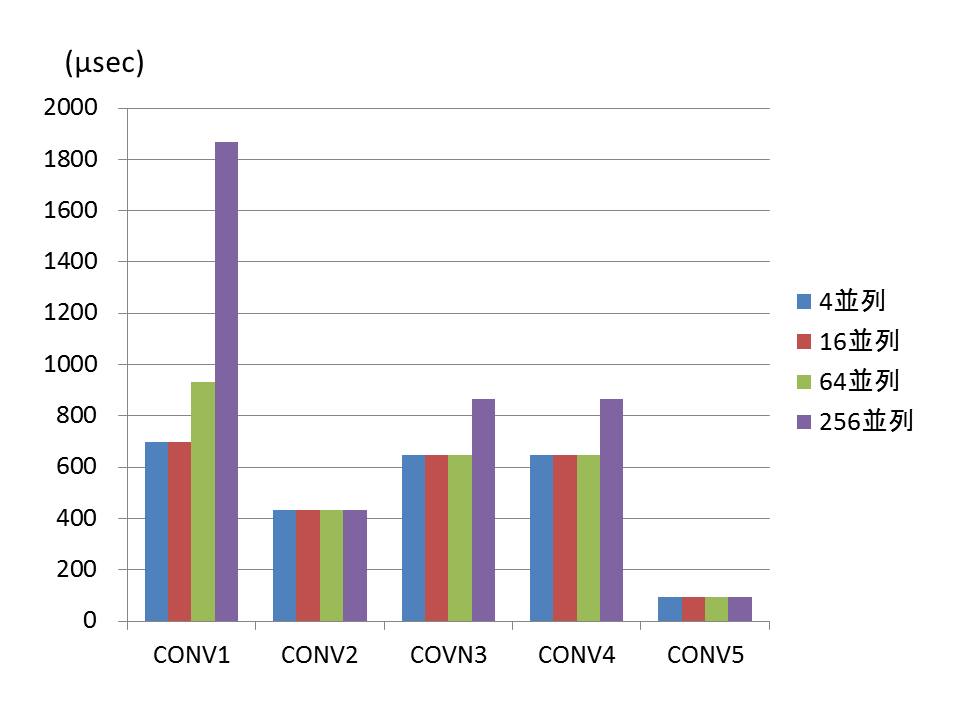
\includegraphics[width=1.0\columnwidth,bb=0 0 720 540]{img/broadcast_time.png}
  \caption{畳み込み層の特徴マップ共有にかかる通信時間($\mu$sec)の予測}
%  \ecaption{Static analysis result of an example pattern}
  \label{gra_broadcast_time}  
 \end{center}  
\end{figure}

\begin{table}[ht]
 \begin{center}
  \caption{特徴マップ共有の予測通信時間($\mu$sec)}
   \begin{tabular}{|c|c|c|c|c|} \hline
     層 & 4並列 & 16並列 & 64並列 & 256並列 \\ \hline
     CONV1 & 699.84 & 699.84 & 933.12 & 1866.24 \\
     CONV2 & 432.64 & 432.649 & 432.64 & 432.64 \\
     CONV3 & 648.96 & 648.96 & 648.96 & 865.28 \\
     CONV4 & 648.96 & 648.96 & 648.96 & 865.28 \\
     CONV5 & 92.16 & 92.16 & 92.16 & 92.16 \\
     FC6 & 40.96 & 40.96 & 40.96 & 40.96\\
     FC7 & 40.96 & 40.96 & 40.96 & 40.96\\
     FC8 & 10.00 & 10.08 & 10.24 & 10.24\\ \hline
  \end{tabular}
  \label{tdmtime}  
 \end{center}
\end{table}

\section{FiC-SW1ネットワークの通信帯域改善のための手法}
STDMによるサーキットスイッチングネットワークでは、通信の帯域を保証できるというメリットがあるが、ノード数が増えると
1ノードに与えられる通信帯域が極端に狭くなってしまうという問題が発生する。

時分割多重のスロット数を減らすことができれば、1スロットを複数のノードで共有する方針で、帯域を改善させることができる。
その単純な方法としては、データのヘッダ情報として、ラベルを定義する方法がある。
スロットを共有しているノードにはそれぞれ固有のラベル番号を振り、送信の際には自身のラベル番号と共にデータを送信するように設計することで、
帯域を狭めることなく疑似的にスロット数を増やすことが可能である。ただし、この帯域の改善方法では
1ノードがスロットを占有している間、そのスロットを共有している他のノードは送信を行うことができない。
そのため、各ノードのスロット占有時間が短い場合でないと有効に働かないと考えられる。

\chapter{畳み込みアクセラレータの実装}
\section{概要}
この章ではFiC-SW1ボード上のFPGAに実装される畳み込みアクセラレータについて解説を行う。
この畳み込みアクセラレータは、図\ref{fig_cnn_on_sw1}のような並列畳み込み演算をより効率的に行う目的で実装する。
アクセラレータの大まかな設計としては、図\ref{fig_cnn_on_sw1}の処理と同様に、前の層からすべての特徴マップを入力として受け取り、分割された重みデータで並列演算し、
次の層へ特徴マップを出力するという方針を取る。

また、アクセラレータ内のすべての特徴マップ・重み・バイアスのデータは32bitの浮動小数点数で扱うものとする。

FPGA上の演算・メモリのリソースは有限なため、効率的にリソースを使用して実行サイクル数を減らさなくてはならない。
今回の設計では、アクセラレータ間でのリソース共有は行わず、各畳み込み層とアクセラレータモジュールは完全な1対1の関係になるものとした。
リソース共有を行うクロスレイヤーな設計では、並列演算性能とリソース消費をトレードオフにすることができるため、リソース消費を抑えた設計を
考える場合には有効である。

\section{アクセラレータモジュール}
図\ref{hw}に、今回実装したアクセラレータモジュールの概略図を示す。アクセラレータモジュールは大きく分けて、演算モジュール、バッファ、入出力ストリームでの3つのパートから構成される。

畳み込み演算の核となる演算モジュールは、パイプライン化された並列積和演算器(PE : Processing Elements)であり、毎サイクル、複数チャンネルの特徴マップを出力できる。
この演算モジュールは、優れた計算効率を出したUCLAのMulti-Layer CNN Accelerator\cite{fpgaopt}の設計を参考にした。

アクセラレータモジュール内のバッファは特徴マップのための入出力バッファと、重みのための重みバッファの2種類がある。
入出力バッファは、自身の演算に必要な特徴マップを格納するためのストレージで、それぞれのバッファはそれぞれの特徴マップをすべて格納できるサイズを持つ。
また、演算モジュールに毎サイクル特徴マップを入出力するために、複数個のバンクに分けることで帯域幅を確保している。
重みバッファはカーネルを格納するためのストレージで、並列化によって分割された重みのすべてを格納できるサイズと、広い帯域幅を持つ。

アクセラレータモジュールの入出力には、Xilinx社のIPであるAXI4-Streamを利用した。AXI4-Streamでは、毎サイクルNbitのデータをストリーム形式で送受信行うことができる。
今回は1サイクルで1個の32bit浮動小数点数データを送受信行える、N=32bitでのストリームとした。

\cite{fpgaopt}では高位合成を用いてスケーラブルに実装可能なアクセラレータの設計を提示している。
リソースと実行時間をトレードオフにすることができる設計を用いることで、リソース制約下で畳み込み演算の並列性を最大限活用でき、
効率的なハードウェアにすることができると考えられる。

\begin{figure}[ht]  
 \begin{center}   
   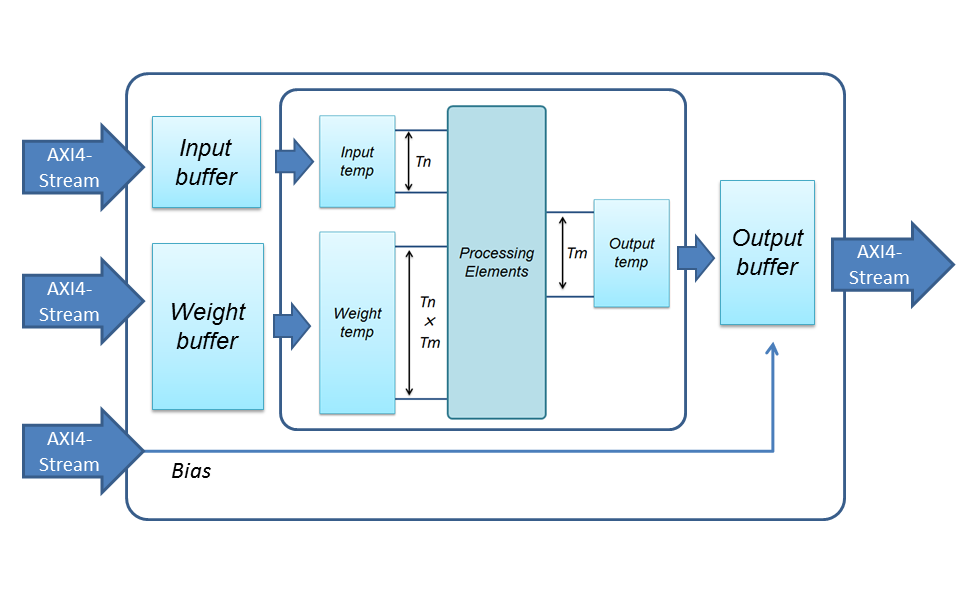
\includegraphics[bb=0 0 720 420, width=1.0\columnwidth]{img/hw.png}
  \caption{アクセラレータの概略図}
%  \ecaption{Static analysis result of an example pattern}
  \label{hw}  
 \end{center}
\end{figure}


 \subsection{演算モジュール}
この節では畳み込み演算の並列性に沿って最適化された演算モジュールを設計する。演算モジュールは、実際に計算を行う並列積和演算器PEsと、そのための一時バッファ(temp buffer)から構成される。

図\ref{pe}は並列積和演算器PEの概要である。図\ref{fig_conv}のように、畳み込み層の特徴のひとつとして、その多くの処理が入力と重みの積和演算から構成されるという点が挙げられる。
この処理の高速化には複数個の積和演算器を並列に配置するのが最も単純で効率的な方法だと考えられる。
したがって、演算モジュールはTn個の入力値からTn×Tm個の重みを用いてT個の出力値を並列に計算できる汎用的な設計となった。
さらに、スループット向上のためにPE内部はパイプライン化されており、毎サイクルTm個の値を出力バッファへと出力することができる。

パラメータTm、Tnはそれぞれ、PEsが同時に扱う入力データ、出力データの数であり、リソース消費量とトレードオフ関係にあるため実装最適化の対象となる。
今回の設計では暫定的に演算モジュールのサイズは(Tm, Tn)=(24, 8)に固定したが、リソース上限によってはこのパラメータを変更することでリソース上限内に消費量を
抑えることが必要となる。

PEsの入出力は演算モジュール内の一時バッファ(temp buffer)に保存される。一時バッファは、入出力バッファ・重みバッファとPEsの間に入り、PEsが入力データTn個、重みTn×Tm個、出力データTm個を高速に
読み書きを行うためのレジスタの役割を持つ。演算モジュール外部から見れば、それぞれ対応する一時バッファのデータを読み書きすることで、計算が行われるという流れになる。

\begin{figure}[ht]  
 \begin{center}   
   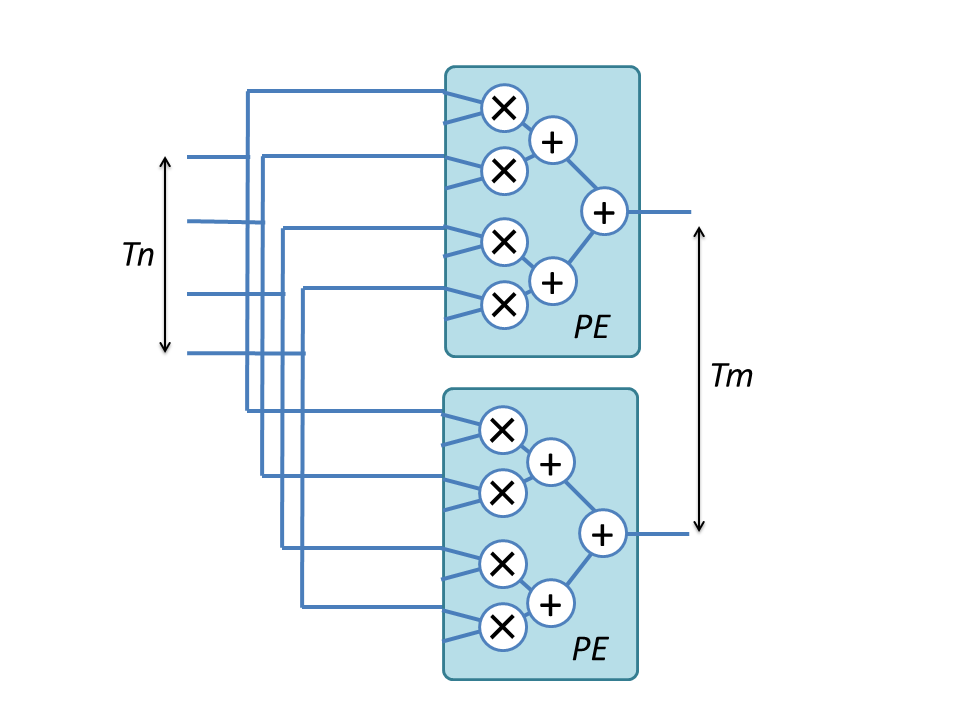
\includegraphics[width=1.0\columnwidth, bb=0 0 720 540]{img/pe.png}
  \caption{並列積和演算器PEs}
%  \ecaption{Static analysis result of an example pattern}
  \label{pe}  
 \end{center}  
\end{figure}
 
\subsection{入出力バッファと重みバッファ}
スイッチモジュールから送られてきた入力特徴マップのデータは、まずFPGA上に確保された入力バッファに蓄えられる。

高速に畳み込み演算を行うためには、演算モジュールは可能な限り広い帯域幅で入力特徴マップにアクセスできなけらばならない。
そこで、入力バッファを特徴マップごとにバンクを分割し並列に読み込むことができるようにした。
これにより、入力バッファと演算モジュールの帯域幅はTn/バンク数となり、帯域幅を改善することができる。
同様の手法で、出力バッファや重みバッファも帯域幅を増減させることができる。。

今回の実装では、入力バッファはTn個、出力バッファはTm個、重みバッファはTm×Tn個に分割することで、最大となるような帯域幅を確保した。
これにより、演算モジュールが毎サイクル、畳み込み演算を行う効率的な機構を実現した。
ただし、この実装を行う場合、バンク数に応じてFPGAリソース消費量が増大するため、過剰なバンク分割によってリソースを浪費することに注意しなければならない。

図\ref{fig_buffer}に、入出力バッファ・重みバッファを演算モジュールと接続した概略図を示す。バッファが特徴マップの次元数によって、
入力バッファはTn個、出力バッファはTm個、重みバッファはTm×Tn個のバンクに分割されている様子がわかる。

\begin{figure}[ht]  
 \begin{center}   
   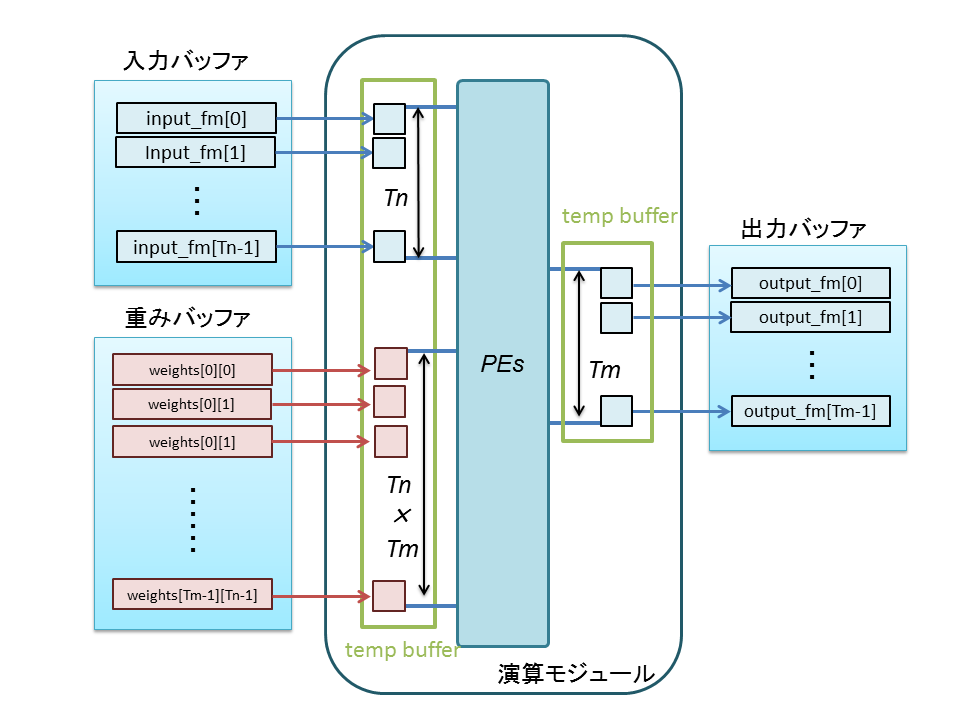
\includegraphics[width=1.0\columnwidth, bb=0 0 720 540]{img/buffer.png}
  \caption{入出力バッファ・重みバッファと演算モジュールの接続}
%  \ecaption{Static analysis result of an example pattern}
  \label{fig_buffer}  
 \end{center}  
\end{figure}
\chapter{アクセラレータの評価}
\section{評価環境}
今回実装するアクセラレータは表\ref{evalu}に示す環境で設計を行い、評価を行った。
Vivado HLSはXilinx社の提供する高位合成ツールで、畳み込みアクセラレータのシミュレーションは
このツール上で行った。評価ボードとFPGAにはFiC-SW1ボードのものと同様にKintex UltraScale XCKU095を用いた。

また、比較のためにCPUで畳み込み演算のソフトウェア実行を行った。そのときのソフトウェア実行環境を表\ref{evacpu}に
示す。

\begin{table}[ht]
 \begin{center}
  \caption{CNNアクセラレータの評価環境}
   \begin{tabular}{|c|c|} \hline
     ツール & Vivado HLS Version 2016.1 (Xilinx) \\ \hline
     評価ボード & Kintex UltraScale XCKU095 (Xilinx) \\ \hline
     FPGA & XCKU095-FFVB2104 (Xilinx) \\ \hline
  \end{tabular}
  \label{evalu}  
 \end{center}
\end{table}

\begin{table}[ht]
 \begin{center}
  \caption{ソフトウェア実行環境}
   \begin{tabular}{|c|c|} \hline
     CPU & Intel Core i5-4250U \\ \hline
     動作周波数 & 1.30GHz \\ \hline
     コンパイラ & GCC 4.4.7 20120313 \\ \hline
  \end{tabular}
  \label{evacpu}  
 \end{center}
\end{table}

\section{アクセラレータのクロックサイクル数とリソース消費量}
演算モジュールの演算器サイズを(Tm, Tn)= (24, 8)としたときの各畳み込み層の計算時間を測定した。
Tmは畳み込み層5層のなかでのMの最大値である24を、Tnは予想されるリソース消費量が上限以下になるように暫定的に決定した。
表\ref{tdmtime}からノード数を16より大きくすると通信時間が増えることがわかるため、今回の実装では通信時間が最小の条件下でノード数が最も高い16並列時を取り扱う。

表\ref{cnnexe}は、CONV1からCONV5を16並列で計算した際のサイクル数の結果となる。
特に、入出力特徴マップのサイズが大きく、次元数が低いCONV1が508118サイクルと最もクロックサイクル数が大きい。
今回のアクセラレータは入出力の特徴マップの次元数以上に処理を並列化していない設計のため、このような結果となったと考えられる。

また、このときのリソース消費量を図\ref{gra_resource}に示す。表\ref{resource}は図\ref{gra_resource}の詳細な結果である。
それぞれの畳み込み層のアクセラレータのリソース消費量は上限に収まっているため、(Tm, Tn)=(24, 8)の演算モジュールのサイズは(最適とはいかないまでも)妥当な値であったと言える。
ただし、単純にアクセラレータを5層分実装するにはリソースが足りないため、各アクセラレータの(Tm, Tn)を調節して規模を縮小させるか、リソース共有を行うクロスレイヤーな設計を考える必要がある。

\begin{table}[ht]
 \begin{center}
  \caption{16並列時の畳み込みアクセラレータの演算サイクル数}
   \begin{tabular}{|c|c|} \hline
     & サイクル数 \\ \hline
     CONV1 & 508118 \\
     CONV2 & 409746 \\
     CONV3 & 166554 \\
     CONV4 & 245434 \\
     CONV5 & 242506 \\ \hline
  \end{tabular}
  \label{cnnexe}  
 \end{center}
\end{table}

\begin{table}[ht]
 \begin{center}
  \caption{16並列時の畳み込みアクセラレータのリソース消費量}
   \begin{tabular}{|c|c|c|c|c|} \hline
     & BRAM 18K & DSP48E & FF & LUT \\ \hline
     CONV1 & 903 & 32 & 11388 & 181047 \\
     CONV2 & 496 & 66 & 80886 & 249112 \\
     CONV3 & 664 & 98 & 135466 & 290533 \\
     CONV4 & 736 & 98 & 152868 & 321012 \\
     CONV5 & 504 & 66 & 119670 & 244851 \\ \hline
     Avaiable & 3360 & 768 & 1075200 & 537600 \\ \hline
  \end{tabular}
  \label{resource}  
 \end{center}
\end{table}

\begin{figure}[ht]  
 \begin{center}   
	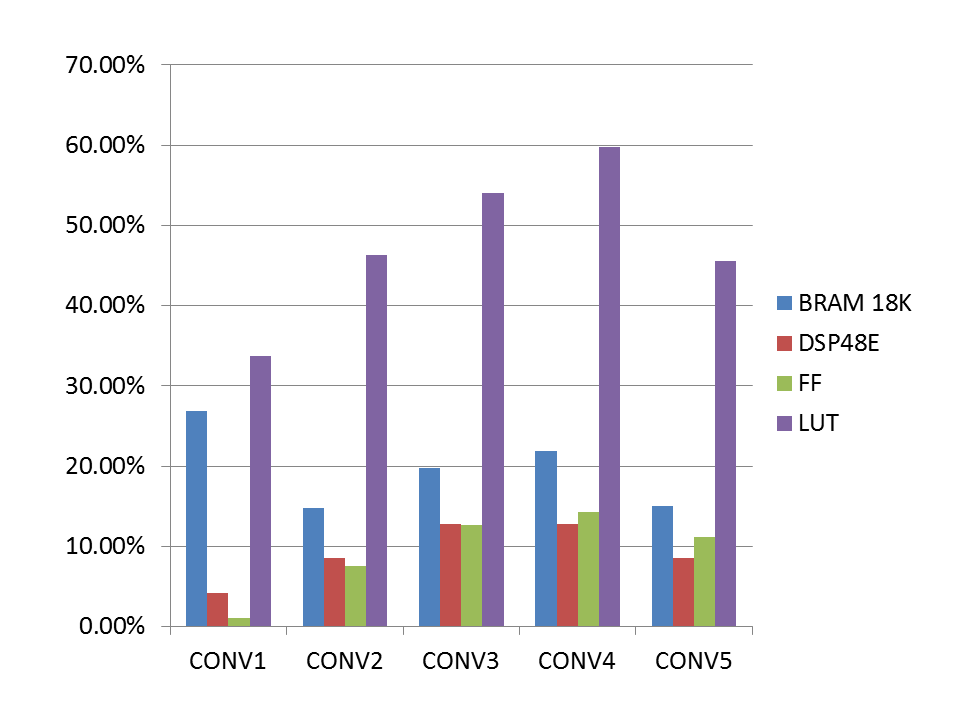
\includegraphics[width=1.0\columnwidth,bb=0 0 720 540]{img/resource.png}
  \caption{16並列時の畳み込みアクセラレータのリソース割合}
%  \ecaption{Static analysis result of an example pattern}
  \label{gra_resource}  
 \end{center}  
\end{figure}


\section{FiC-SW1での畳み込み層の計算時間と通信時間}
FiC-SW1上のKintex UltraScale KU095は100MHzで動作するため、クロックサイクル数から計算時間を計算できる。表\ref{cnnexe}と表\ref{tdmtime}から、16並列時の畳み込み層の計算時間と通信時間の比較を、図\ref{gra_time}に算出した。
表\ref{timecomp}は図\ref{gra_time}の詳細な結果である。
通信時間に対する計算時間の比率は、約2倍から約10倍、CONV5から識別層FC6の間では約26倍になるという結果になった。CONV5の比率が高くなっているのは、CONV5からFC6の間でプーリング層POOL5によって
特徴マップのデータが大幅に削減され、特徴アップ共有の通信にかかる時間が短縮されたことが原因である。

通信時間の計算には、ネットワークのトポロジ、スイッチの遅延、ヘッダ付与による帯域減少は考慮していないため、実際の通信時間は今回の試算より大きくなると予測される。
また、今回のアクセラレータは単純な設計なため、より複雑で高性能な設計(ストリーム機構の見直し、ダブルバッファの導入など)を施すことで実行サイクル数も小さくできる可能性が残っている。
それに伴って通信時間に対する計算時間の比率も小さくなると推測される。

計算時間と通信時間の合計が畳み込み演算の実行時間である。図\ref{gra_cputime}では、今回のFiC-SW1の畳み込みアクセラーレータでの実行時間と、一般的なCPUやUCLAのマルチレイヤー
CNNアクセラレータでの実行時間と比較した。表\ref{cputime}は図\ref{gra_cputime}の詳細な結果である。CPUでのソフトウェア実行は表\ref{evacpu}に従い、Intel Core i5-4250U(1.60GHz)を使用した。FiC-SW1の畳み込みアクセラレータは、CPUに比べて658倍高速であることがわかる。
これはUCLAの設計\cite{fpgaopt}と比べて半分程度の性能に留まる。しかし、今回の設計ではUCLAが行っているような演算器サイズやバッファリングの最適化は一切行っておらず、
これを行うことで性能が大きく向上する可能性が残っている。アクセラレータの最適化は今後の重要な課題とする。

\begin{table}[ht]
 \begin{center}
  \caption{16並列時の通信時間に対する計算時間の比率}
   \begin{tabular}{|c|c|c|c|} \hline
     &  計算時間($\mu$sec) & 通信時間($\mu$sec) & 比率 \\ \hline
     CONV1 &  5081.18 & 699.84 & 7.26 \\
     CONV2 &  4097.46 & 432.64 &  9.47 \\
     CONV3 &  1665.54 & 648.96 &  2.57 \\
     CONV4 &  2454.34 & 648.96 &  3.78 \\
     CONV5 &  2425.06 & 92.16 &  26.31 \\ \hline
  \end{tabular}
  \label{timecomp}  
 \end{center}
\end{table}

\begin{table}[ht]
 \begin{center}
  \caption{畳み込み演算の実行時間}
   \begin{tabular}{|c|c|c|c|} \hline
     &  CPU(msec) & UCLA\cite{fpgaopt}(msec) & FiC-SW1(msec) \\ \hline
     CONV1 & 1110 (192.01x) & 3.66 (0.63x) & 5.78 \\
     CONV2 & 5170 (1141.26x) & 2.37 (0.52x) & 4.53 \\
     CONV3 & 1520 (656.73x) & 1.60 (0.69x) & 2.31 \\
     CONV4 & 2530 (815.26x) & 1.20 (0.39x) & 3.10 \\
     CONV5 & 1670 (663.43x) & 0.80 (0.32x) & 2.52 \\ \hline
     Sum & 12000 (657.67x) & 9.64 (0.53x) & 18.25 \\ \hline
  \end{tabular}
  \label{cputime}  
 \end{center}
\end{table}

\begin{figure}[ht]  
 \begin{center}   
	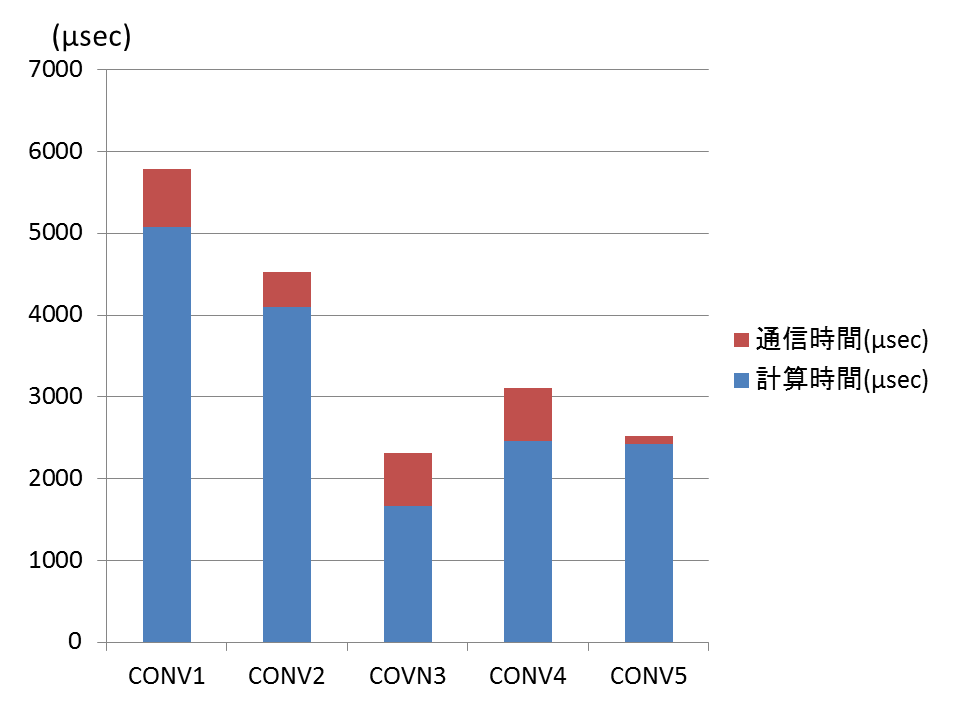
\includegraphics[width=1.0\columnwidth,bb=0 0 720 540]{img/time.png}
  \caption{16並列時の畳み込み層の計算時間と通信時間の比較}
%  \ecaption{Static analysis result of an example pattern}
  \label{gra_time}  
 \end{center}  
\end{figure}

\begin{figure}[ht]  
 \begin{center}   
	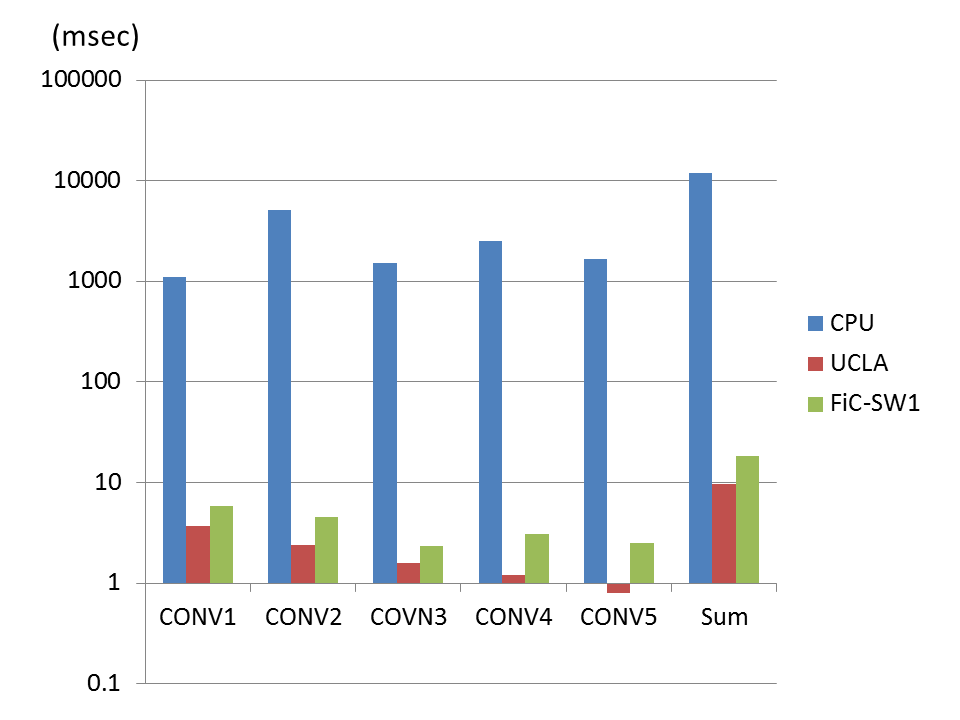
\includegraphics[width=1.0\columnwidth,bb=0 0 720 540]{img/cputime.png}
  \caption{畳み込み演算の実行時間の比較}
%  \ecaption{Static analysis result of an example pattern}
  \label{gra_cputime}  
 \end{center}  
\end{figure}



\chapter{結論}
FiC(Flow-in-Cloud)システムは、NEDO人工知能プロジェクトにおいて、FPGAノード、GPUノード、メモリノードなどの異種ノードを多数組み合わせた大規模計算システムである。
このFiCシステム上で、スイッチノードしての役割を持つFiC-SW1は高速リンクを多数接続したFPGAボードである。
本稿では、このFiCシステム上でスイッチノードとしての役割と、初期のソフトウェア開発用テストベッドの役割を持つFiC-SW1をボードの計算性能と転送性能の
予備評価を行う目的で、大規模CNNのAlexNetをベンチマークとして、畳み込み演算の並列性について検討し、FIC-SW1上のFPGAに並列に畳み込み演算を行う畳み込みアクセラレータを実装した。

その結果、最適化を施していないアクセラレータでも一般的なCPUに比べて658倍高速化することに成功した。また、
通信時間に対する計算時間の比率は、2倍から10倍、最大で26倍になることがわかった。
ただし、通信時間の算出ではヘッダや通信遅延などを考慮していないため、実際の比率はこれより小さくなると予測される。

以下に今後の課題を述べる。本稿では、並列化・高速化の対象をCNNの畳み込み層の畳み込み演算のみに限って検証を行ったが、
CNNのプーリング層、正規化層、識別層についてもどのように並列化・高速化を行うか検討しなければならない。
また、今回実装した畳み込みアクセラレータは比較的単純な構造をしており、ダブルバッファリングなどの手法によってさらなる低リソース化・
高速化できる余地が残っている。アクセラレータを単純に5つ実装するにはリソースが足りないため、アクセラレータの改良やFPGA内でリソース共有を
行うことも検討する必要もある。


%% \input{chap7/chip-eval.tex}
%% \chapter{まとめと今後の課題}
{
\label{chap:conclusion}
\section{結論}
\label{sec:conclusion}
VPCMAにおいて、実行するアプリケーションと要求性能に応じて電力を最小化するパイプライン段数とボディバイアス電圧を決定する手法を検討した。トレードオフの複雑さから単純に計算することが困難であったため探索はブルートフォースで行った。4つの24bit画像処理アプリケーションを実行するシミュレーションを行い評価を行った。

パイプライン段数に着目するとVPCMAおいてはアプリケーションや要求性能によらず全段にパイプライン分割した場合がもっとも電力が小さいとわかった。この結果はVPCMA特有のものであり、ブルートフォース探索によってによって明らかとなったアーキテクチャの特徴とも言える。このように本手法ではアーキテクチャに依存せずに電力を最小化するパイプライン段数を求めることができた。

ボディバイアス制御の粒度を行単位とすることによる効果をボディバイアス制御をしない場合、制御の粒度をPE\_ARRAY全体とした場合との比較を行うことにより検討した。
ボディバイアス制御をしない場合と比べて平均約46\%の電力削減率が得られた。一方で一律制御と比べると電力削減率は平均0.80\%であった。しかし、要求性能が高くなるにつれて行単位の制御では一律制御に対して高い電力削減率を示し、その効果はアプリケーションと要求性能に依存することがわかった。

\section{今後の課題}
\label{sec:future}

本論文で検討した手法にはブルートフォース探索を採用していることはすでに述べた。そのため、パイプライン分割のパターンを制限してもパイプライン段数とボディバイアス電圧を決定するのに時間がかかっていた。このようにパイプライン段数は粗粒度に探索を行っているため本研究では想定していないパイプライン分割のパターンの方がより小さい電力を示す可能性がある。ただし、本研究で示されたように電力を最小化する段数は使用している行数の付近にあるはずであり、探索はその周辺を行えばよい。よって、本論文で提案した手法のアルゴリズムには改良の余地がある。例えば遺伝的アルゴリズムなどを代表とする進化的計算アルゴリズムを採用し得られる結果と本研究のブルートフォース探索の結果を比較することにより、この手法に適するアルゴリズムを検討する必要があると考えられる。

アプリケーション依存性があるということは、どのPEにどの演算をマッピングするかに依存するということである。本研究ではアプリケーションのマッピングは固定したままでパイプライン
段数とボディバイアス電圧を変化させて電力を見積もり最小のものを探索していた。しかし、各々のパイプライン段数、ボディバイアス電圧に対する適切な演算のマッピングは異なる可能性がある。したがって、演算のマッピングを変化させた場合の影響についても評価を行う必要があると考えられる。
}

\chapter*{謝辞}
本研究を行うにあたり、慶應義塾大学の天野英晴教授には懇切なご指導ご鞭撻を賜りましたこと心より感謝いたします。
天野教授には主査も行っていただきました。

同研究室の志村英樹先輩には副査を行っていただいた他、高位合成ツールの使い方のご教授をはじめ、大変お世話になりました。

また、この成果(の一部)は、国立研究開発法人新エネルギー・産業技術総合開発機構(NEDO)の委託業務の結果得られたものです。

プロジェクト内で多岐にわたりご指導いただいた東京大学の工藤知宏教授、国立情報学研究所の鯉渕道紘教授に深く
お礼申し上げます。今回、NEDO人工知能プロジェクトに関わることができ大変光栄に思います。

%-end body-----------------------------------------%


%-reference----------------------------------------%
\bibliographystyle{junsrt}
\bibliography{main}
%-end reference------------------------------------%
\end{document}
